
\documentclass[11pt,letterpaper]{article}
\usepackage[latin1]{inputenc}
% Choose C-x f RET latin-1 to save this file in Emacs
\usepackage[left=3cm,top=2cm,right=4cm,bottom=3cm,nohead]{geometry}
\usepackage{graphicx}
\usepackage{html}
\usepackage{rotating}
\usepackage{palatino}

\renewcommand{\sfdefault}{uop}
\usepackage{sectsty}
%\allsectionsfont{\sffamily}

%\renewcommand{\~}{{\raise.17ex\hbox{$\scriptstyle\sim$}}}
\renewcommand{\~}{{ \leavevmode\raise.17ex \hbox{$\scriptstyle\sim$}}}

% \author{David Reitter and Kevin Walzer}
\title{
\includegraphics[]{aquamacs-logo.pdf}\\
Manual}

\hypersetup{pdftitle={Aquamacs Emacs Manual}
pdfpagemode=FullScreen,
colorlinks=true, linkcolor=blue}

\newcommand{\ttfile}{\tt}

\begin{document}

\sffamily\maketitle
\rmfamily

\tableofcontents
\pagebreak


\section{Aquamacs Emacs: a User-friendly Emacs Distribution}

Aquamacs is an freely-available build of the powerful
Emacs text editor
(\url{http://www.gnu.org/software/emacs/emacs.html}) adapted to the Mac.

\emph{Made for Mac} means that Aquamacs is easy to use for anyone used to the macOS operating system, that is, Aquamacs adopts the way the mouse and the keyboard are used to interact with windows and text in other Mac programs.  However, Aquamacs remains \emph{GNU Emacs}, the text editor of legendary power and configurability.  Given Emacs' almost 45-year history, it is unsurprising that Emacs has evolved to have an enormously complex interface that, while consistent across platforms, is usually at odds with the specific interface conventions of the particular platform on which it is being used. The original GNU version of Emacs for the Mac, called Carbon Emacs, is no different, neither are other currently available builds of GNU Emacs on the Mac.

Aquamacs Emacs implements the standard OS X keyboard shortcuts and other interface conventions, integrating Emacs into the MacOS environment to a far greater degree than other versions of Emacs.  We refer to this experience as \emph{Aqua}, the name given to the graphical user interface by Apple at an early point in the Mac's product lifespan.  Our integration allows Mac users who might be unfamiliar with Emacs' complex standard interface to harness its amazing editing power in a familiar way. For users familiar with Emacs, Aquamacs provides some settings to make it more or less Emacs-like.

\begin{figure}
\centering
{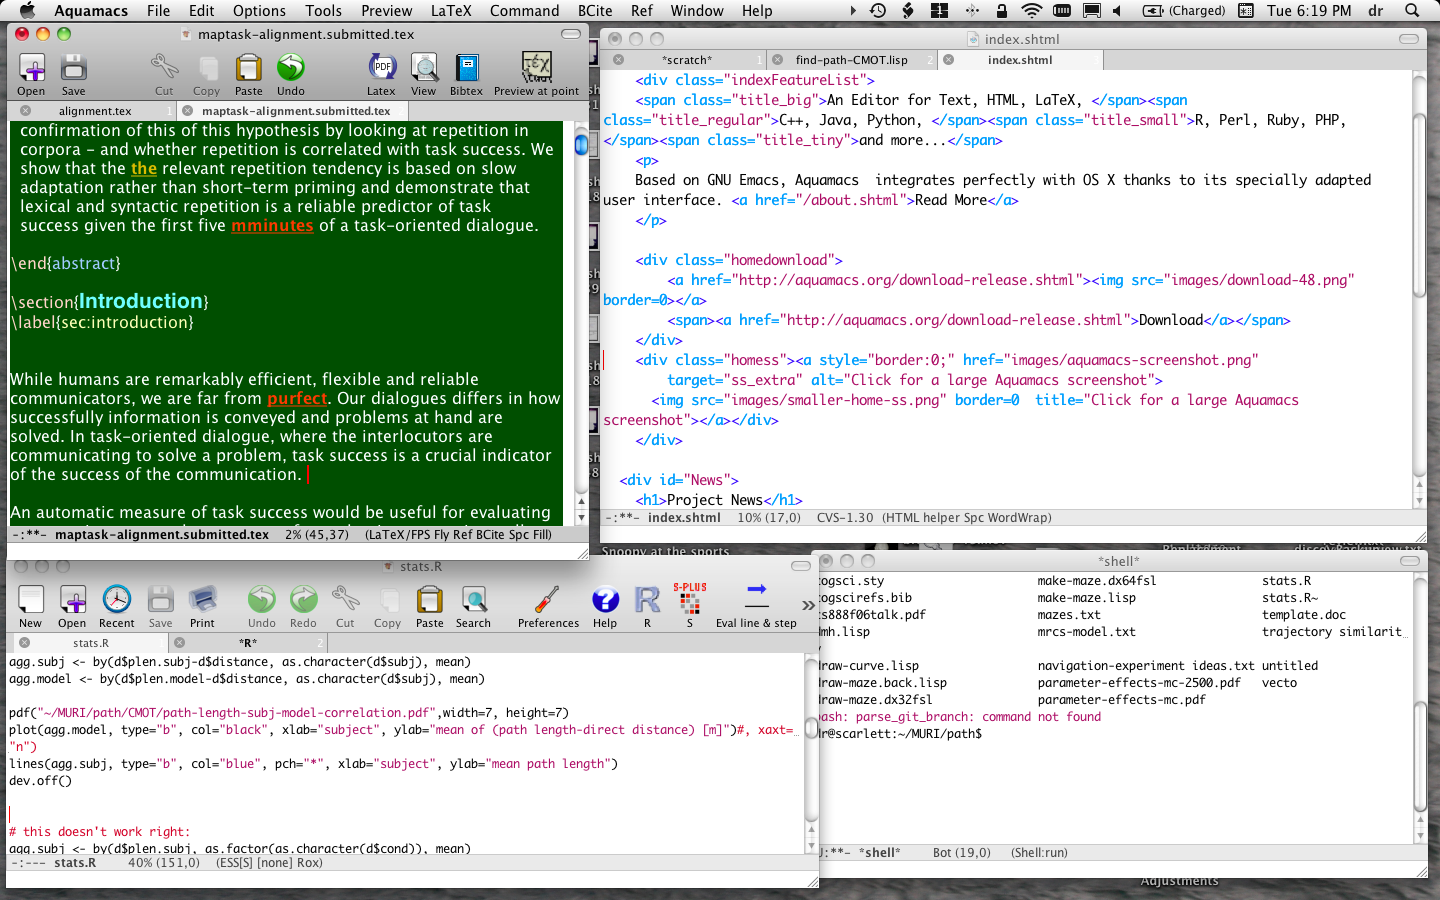
\includegraphics[width=5in]{aquamacs-screenshot.png}}
\caption{Aquamacs combines the legendary power of Emacs with
  user-friendly customizations to provide a more Aqua-specific user experience.}
\label{aquamacs-screenshot.jpg}
\end{figure}

You can always download the latest version of Aquamacs from the project home page, \url{http://aquamacs.org}.  Just download the disk image (DMG), move the Aquamacs application bundle to your hard drive, and launch.


This documentation aims to introduce Aquamacs to novice users of Aquamacs Emacs, to help them get started with this powerful text editor. The documentation also aims to introduce Aquamacs to experienced users of Emacs, who may find aspects of its interface inconsistent with their experience.

The Aquamacs documentation will focus on the following areas:

\begin{itemize}
\item Tutorial: Aquamacs for Beginners
\item In-Depth: The Aquamacs Interface
\item Aquamacs for Emacs Veterans
\end{itemize}

Our hope is that using Aquamacs will be a rewarding experience both for new users, who come to appreciate the power of Emacs without the steep learning curve, and for experienced Emacs users, who may find Emacs' integration into the Aqua environment an unexpectedly pleasant surprise.

\subsection{Terminology in this Manual}

GNU Emacs uses a terminology that is different from what users of modern, graphical environments are used to. Windows become \emph{frames}, and documents are held in \emph{buffers}. We will concentrate on the Emacs terminology in this manual in places where this is not confusing.

Aquamacs Emacs is an extensive \emph{distribution} of GNU Emacs with modified defaults -- almost up to the point where it could be called a \emph{fork} - a completely new program. However, Aquamacs always contains the latest version of GNU Emacs. It is useful to understand the relationship between Emacs and Aquamacs. In this manual, we will use the term \emph{Emacs} to refer to the core which is used on many different operating systems and built and distributed by the GNU Project. We will use the term \emph{Aquamacs Emacs} (or just \emph{Aquamacs}) to refer to the present implementation.



\section{Tutorial: Aquamacs for Beginners}

\subsection{What Makes Aquamacs Like Other Text Editors}
When you first launch Aquamacs, you will see that it is like many other text editors: you can type text, cut and paste text, and save and close a file using the menubar or standard OS X keyboard shortcuts (Command-S for save, Command-X for cut, Command-V for paste, and so on). If you are writing one of the many text formats that is supported by Aquamacs, such as HTML, you will also note Aquamacs' use of \textit{syntax coloring,} which sets certain parts of the text---such as HTML markup---in a different color than the text content. This makes editing the text and adjusting the markup easier.

If you are used to the way Emacs does things, you may be surprised about how Aquamacs works:  Aquamacs differs significantly from Emacs.  While the useful Emacs key bindings are supported and Emacs packages usually just work, Aquamacs is adapted to be comparable to younger text editors (than Emacs).  It also comes with a range of packages that give you greater comfort in editing certain types of files.


\subsection{What Makes Aquamacs Emacs Different from Other Text
  Editors} If you look at some of the menu items and keyboard shortcuts, you will see some of the features that make Emacs different from other text editors. Although Aquamacs has been designed to present many of these features in an Aqua-friendly way, it does not hide these features. Aquamacs is a complete editing environment.

\begin{itemize}

\item \textbf{Sophisticated text processing.} Aquamacs features text
  editing capabilities that go far beyond the average text editor. For
  instance, Aquamacs features several kinds of search and replace: it
  can replace text incrementally, it can search and replace text by
  complex patterns of characters (regular expressions) and not just by
  word matching, and so on. Aquamacs also features support for
  virtually every kind of text file imaginable: computer code such as
  C/C++, HTML, \LaTeX, XML, and other formats.
\item \textbf{Buffers.} One of the features that makes Emacs such a productive editing
environment for experienced users is the concept of \textit{buffers.}
A buffer is, simply said, a document that is being edited. It can be
displayed in any window, and you can even display a buffer twice. But
buffers don't just hold text files. They can hold messages from a
program that's running, they can be shown in a window that you can use to
actually send commands that Aquamacs executes, and other functions. The
Buffers menu in Aquamacs Emacs allows you to switch quickly between
windows, to send execute or preview the code you are writing with a
couple of keystrokes, and to monitor logs of commands you are
executing.
\item \textbf{Integration with additional tools.} Aquamacs' ``Tools''
  menu provides access to file comparison and version control,
  compiling and debugging of program code, the ability to read e-mail
  and newsgroups, and more.

\end{itemize}

In addition to its large number of features, Aquamacs also defines
some interface terms differently than other OS X applications. See
Table \ref{tab:terms} for more information.


\begin{table}[t]
\begin{center}
\begin{tabular}{|c|c|}
\hline  OS X Term & Emacs Term  \\
\hline  Window &  Frame \\
\hline  Tab/pane  &  Window \\
\hline Document &  Buffer \\
\hline Cursor  & Point \\
\hline Mouse pointer & Pointer \\
\hline Keyboard shortcut &  Key (binding)\\
\hline
\end{tabular}
\caption{Key Emacs terms and their Apple counterparts.}
\label{tab:terms}
\end{center}
\end{table}

This list provides just a small sample of the functionality
available in Emacs. Aquamacs' customizations make Emacs much easier to
learn; it is possible to get started and become productive
quickly. However, harnessing all of Emacs' power, even with assistance
from the familiar Aqua user interface, will take time.



\section{In Depth: The Aquamacs Interface}

In this section, we will walk through the Aquamacs interface step by step, and will introduce relevant points about how Aquamacs Emacs solves particular editing problems in a distinctive way. We will specifically emphasize the functions that Aquamacs offers as opposed to GNU Emacs, which readers might be familiar with anyways.

\subsection{Tabs and Windows}
Aquamacs has an optional tabbed interface for organizing multiple open buffers. A tab is a GUI handle for a particular buffer. If you have ``Show Tabs'' checked in the Options menu, then each displayed buffer and any buffers that are subsequently created will be associated with a tab in the tab bar, just above the text area. (Note that the tab bar is hidden whenever it would display only a single tab. You may want to turn off ``Show Buffers in New Frames'' in the Options menu, in order to get full benefit from tabs.) If the tab bar cannot display all tabs at once, scroll bars appear to allow you to choose the displayed subset of tabs. Additional tab-related functions are available from the Window menu and from the tab bar's context menu.

Tabs in Aquamacs do not act like containers -- one can't open a file in an existing tab. (This is in contrast to tab implementation in a number of popular internet browsers.) Rather, tabs provide a convenient way to navigate existing buffers. Because Emacs allows you to simultaneously display the same file in multiple windows or frames, it is possible to have multiple tabs (in different windows) that are associated with the same buffer.

To access tabs quickly, the key commands A-M-0,1,2 through 9 may be used; A-M-1 (normally: Command-Option-1) will select the first, leftmost tab in the window.\footnote{Use the function `tabbar-define-access-keys' to configure the keys in your {\tt Preferences.el} file.}

Note that Tab functionality may be impaired in modes that use the Emacs Header Line.  This includes the Buffer List (C-x C-b) and \emph{psvn}.

A related option lets Aquamacs open new buffers in their own, extra frames.  The option may be combined with Tabs, when you want to create tabs manually (Command-T), but visit new files in separate windows.  Normally, we would not recommend to combine the two options.

Note that when tabs are switched on, or when buffers are shown in new frames, then closing a window has a different implication: it will remove the buffer from memory (in Emacs terminology, it will \emph{kill} the buffer).  In case there are unsaved modifications, you will be asked whether you'd like to save them.
If neither tabs nor ``Show Buffers in New Frames'' is on, then closing a window using Command-W, or closing a whole frame with the red closer button has no such implication.  The buffer remains in memory and is available from the Window menu.  It is not automatically saved.

\subsection{Configuring the Toolbars}

The easiest way to set up icons in the toolbars is to right click on the toolbar that you'd like to customize and select \emph{Customize Toolbar...}.  This will show a panel with all available icons.  Drag and drop those into the toolbar.

Note that if a mode provides its own set of icons or additional icons, Aquamacs will store a separate configuration for that toolbar.  This way, you can set up toolbars for different tasks.  (Note that if modes, perhaps after an upgrade, add or remove icons, Aquamacs will adopt a new customization set for the toolbar.)

Click on the button in the top right corner of the frame to remove the toolbar completely.  Use the menu items \emph{Options / Appearance / Adopt Face and Frame Parameters as Default} and \emph{Options / Save Options}  to make this change stick.


\subsection{File}
The File menu includes basic operations for opening, closing, and printing files. Opening and saving files uses standard Mac keyboard shortcuts (Command-O, Command-S), and uses standard Aqua dialog boxes.

You can create a new buffer: Aquamacs allows you to choose from a list of recently and commonly used editing modes.  A similar function lets you change the current editing mode.

You can also open a directory. When called by mouse from the menubar, this brings up a standard Aqua dialog box. When called up with a keyboard command (C-x d), it brings up a directory name in the ``minibuffer'' (small space for commands at the bottom of the main window, or frame).

Printing is fully supported, although no ``Page Setup'' option is available at this point.  You will see a print screen (in the system's Preview.app) from where you can select a printer and the usual options.  This may take a few seconds to appear with very large buffers. (Printing of embedded images such in LaTeX Preview mode is currently not supported.)

You may export your buffer to PDF or to HTML format. This operation
preserves all the formatting, including any word-wrapping - so you may
want to choose a font and resize the frame so that the lines are
wrapped in the intended way (if Soft Wrapping is used).

The paper size for printing and PDF export can be configured by customizing the variable `ps-paper-type' (use Options / Customize Aquamacs / Specific Option).

\subsection{Edit}
The Edit menu is the heart of Aquamacs' textual wizardry. Aquamacs supports
all customary editing functions, such as cut, copy, paste, and simple
search and replace. In Aquamacs these basic functions are supported by
standard Aqua keyboard shortcuts. There is a great deal more
functionality, however, than the average text editor. For instance,
Aquamacs Emacs allows you to go to a specific line number in the file you are
editing, to the top or bottom of the buffer, and so on. It also supports searches with \textit{regular
expressions,}
which are sophisticated text patterns that go beyond simply matching a
specific set of characters (or ``string''). Aquamacs Emacs also stores more
than twenty of the most recently-copied items on the clipboard, and
these are accessible from the menu in case you need to paste these
items again.  The Edit menu also supports ``bookmarks,'' a feature
that allows you to save your place in a specific file.

Aquamacs lets you spell-check your texts, either while typing (`flyspell-mode') or for the whole buffer with an interactive interface (`ispell').


\subsection{Options}
The Options menu is where you can easily customize your
settings. The options that you can configure include syntax coloring,
matching of parentheses (useful for text markup that depends on open
and close brackets), how to display buffers and frames, fonts, and other
settings. For more information on fonts, please see Section \ref{Look}.

If you want to delve deeply into customizing Aquamacs, select
``Customize Emacs:Top-Level Customization Group'' in the Options
menu. A new frame titled ``Customize Group: Emacs'' will open. Scroll
down and find the ``Aquamacs Group'' listing, and push the ``Go to
Group'' button. This will open a new frame with all of the
configuration options for Aquamacs ---power users can customize Aquamacs this way, or via the Emacs Lisp programming language, elisp---and each option is documented there.
Table \ref{tab:variables} displays a complete list of the options.

\subsubsection{Line wrapping}

Text is usually shown and read line by line.  Several lines commonly form a paragraph.   However, text is not necessarily stored this way in a file:  sometimes, a \emph{line} stored in a file is much wider than what would fit on a computer screen, and is really a paragraph.  This makes sense: authors of documents do not know how wide the reader's computer screen is, or how wide the window is going to be that is used to read and edit the text.  Aquamacs supports this mode of editing with \emph{word wrapping}: lines are wrapped at word boundaries.  This way, a buffer line is displayed as a paragraph (several visual lines) on the screen.  In Aquamacs, this mode of operation is called \textbf{ word wrap} and is available from the Options menu.  Internally, word wrapping enables \emph{Visual Line Mode}.\footnote{Earlier Emacs versions provided `longlines-mode', which is similar, but is unreliable and deprecated.}

What's the alternative?  \textbf{Hard line breaking} means that one line shown on the screen corresponds to one line in the buffer and file.  This means that even if a window is resized, the lines still stay the same, and word wrap will occur in the same place on every machine that displays the file.   Line Breaking, called \emph{Auto Fill} in classical Emacs, changes the actual buffer and file contents, unlike all the other options discussed here.

Long lines can also be \textbf{truncated} (cut off) or be continued (\textbf{wrap}) on the next line.

Line wrapping can be set to Truncate, Wrap, Word Wrap and Line Breaking (auto fill) under \emph{Options / Line Wrapping} for the current buffer.  A \emph{Set as Default} will set it as default for all buffers that have no explicit line wrap setting.

Note that Word Wrapping (`visual-line-mode') affects the function of the cursor movement keys (arrows, and C-a, C-e, C-p and C-n).  In Aquamacs, this can be easily customized.  The default is as such:
\begin{itemize}
\item In Word Wrapping (visual-line-mode), C-aenp and arrow keys move according to visual lines.
\item Without Word Wrapping (visual-line-mode off), arrow keys move visually, but C-aenp move non-visually according to buffer lines as in Emacs 22 and Aquamacs 1.x.
\end{itemize}
You may configure this behavior via the `line-move-visual' customization variable.  Set it to \emph{t} for unconditional visual movement of all keys, and \emph{nil} for unconditional logical (buffer) movement of all keys.

Aquamacs allows you to automatically set the right type of line wrapping for text files using the ``Detect Line Wrap in Text Files'' function.  (You can control the default, e.g.,~for new files, by setting `auto-word-wrap-default-function' to `set-word-wrap' using Options / Customize Aquamacs / Specific Option.)

A useful function to convert hard wrapped text into soft wrapped text can be found in the Edit menu: \emph{Remove Hard Line Breaks} will turn (non-indented!) paragraphs into soft-wrapped lines (turn on soft wrapping to see).

Similarly, to manually reformat text that is laid out line by line, using hard line wraps, use \emph{Wrap and Re-Format}.  Emacs terminology calls this process \emph{filling}.


\subsubsection{Using the Options key and more...}

The keyboard has always been the essential user interface to Emacs -
it's what makes Emacs so efficient as an editor for daily
tasks. There are keyboard bindings for pretty much every task. Many
bindings involve pressing the ``Meta'' modifier key - it's a key just
like Control or Shift, which all go together with another (normal)
key. ``Meta'' has only really existed on Unix keyboards long time ago
-- nowadays, computers have other keys instead. Therefore, you will
need to press another key on your Macintosh keyboard. \emph{By default, this
is the Option key}, but you can use the ESC key instead (in this case,
you may press ESC first, then the rest of the keys).

\paragraph{Inputting characters with the Option key on non-English
  keyboards.} In most non-English keyboard layouts, the Option key
also serves to input characters such as $\{$ or $\backslash$ or
@. Using Option as Meta would inhibit you from inputting those
characters. You have three options to get around this. \emph{Either},
you deselect ``Option Key for Meta'' in the Options menu (under
``Option Key''), in which case you will have to use ESC for Meta,
\emph{or} you toggle back and forth between the modes using Command-;,
\emph{or} you use Option for Meta, but enable one of the emulation
modes provided in the same menu under ``Option Key''.  For those keyboard layouts supported, \textbf{this option is the most convenient}.  The emulation will allow
you to input all common characters with the Option key, while using Option for Meta in general.

Alternatively, Aquamacs allows you to use another modifier key -- such
as the Function key on laptops. The customization group ``Aquamacs''
contains appropriate settings, reachable via the menu items in Options / Customize Emacs.

\subsubsection{Languages of the World - Dealing with Different Character Sets}

Computer keyboards were designed to input text in languages with a
small character set.  Aquamacs Emacs lets you use your keyboard with a
variety of \emph{ input methods } in order to input text in languages
with many characters, among them Asian languages.

By default, Aquamacs uses the standard Mac user interface to input
characters, called ``System Input Method''.

The Multilingual Environment, present in GNU Emacs, provides a number
of predefined input methods.  Aquamacs Emacs extends this: On Mac OS
X, because of the particular ways of user interface and unicode
handling, these standard Emacs language environments are not enough to
read and write some international languages.  One needs to set
additional parameters, especially, the language specific coding
systems.

You can find these new language environments (Korean, Japanese,
Chinese-GB and Chinese-BIG5) -- among other ones -- under "Aquamacs
Multilingual Environment".

\subsubsection{The Right Look: Colors and Fonts for Frames and Modes}
\label{Look}
\label{frame-appearance-styles}
Aquamacs allows you to alter specific features of the current frame
via functions in the Options menu. ``Font for *-mode...'' lets you
choose from the installed system fonts.  You can also choose foreground and background colors.  \emph{ These settings only apply to buffers in the current major mode}, provided \emph{Autofaces} is turned on (as is by default).  Without Autofaces, the settings apply to all frames and set the frame default.

With \emph{Autofaces}, Aquamacs Emacs lets you pick a style specific to the current
mode.  For example, you can use different font settings when you are editing
C or LaTeX, then when you are editing a text file.   Note that all settings not sepcified for the mode are taken over from the default. Specifically, color and font choices are prioritized in this order: {\it 1.} Mode-specific face, {\it 2.} Autoface Default Face, {\it 3.} Frame default.

You can use ``Adopt Frame Parameters as Frame Default'' to accept the appearance of the current frame for future frames; this includes the visibility of the tool bar, fringes, and more (but not position and size).

If you're more of an Emacs expert and you'd like to configure things manually by means of elisp or the customization buffer, configure the following faces. With Autofaces, you can customize the faces directly (via M-x customize-face).  The face name for a major mode is always named after the major mode, e.g. ``latex-mode-default'' is the autoface face for `latex-mode'.  The Autoface default face is named `autoface-default'.
The default for all frames is the `default' face.

You can also customize the variables for the frame default: ``default-frame-alist'' and ``initial-frame-alist'', as documented in the Emacs manual.  You can, alternatively, use ``Adopt Frame Parameters as Frame Default'' to accept the appearance of the current frame for future frames; this includes the visibility of the tool bar.





\subsection{Window}
The Window menu allows you to navigate through the windows and frames that you may have open. Note that a ``buffer'' is not synonymous with a window or frame, in that you can split a frame and have more than one buffer contained within. (Multiple windows/frames is a feature of Aquamacs; standard Emacs does not support this.) In addition to standard frames that display open files, there are a few other important buffer types. One is the ``scratch'' buffer, which is simply a buffer to type notes into; this can also be the starting point for a file to save, and a buffer to type configuration commands for Aquamacs (an advanced feature). Another is the ``Messages'' buffer, which displays a log of output from Emacs commands and operations. Finally, there is the ``info'' buffer, in which Aquamacs Emacs displays built-in user help, tutorials and other documentation in Emacs' ``info'' format.

From the Window menu, you can also open a new ``frame,'', or split the open window into two separate ones.  There are keyboard shortcuts for all of these commands.


\subsection{Tools}
The Tools menu provides access to a variety of functions, including integration with version control systems, running shell commands, searching external files for text, and compiling and debugging software code. The Tools menu also provides access to newsgroups and e-mail.\footnote{The functionality provided in the Tools menu is, to say the least, diverse, and is part of the attraction of Emacs for a large number of users---particularly advanced users. It is not necessary to use Aquamacs as an e-mail client to appreciate its considerable power and utility, however.}

\subsection{Help}
The Help menu contains a wealth of information about Aquamacs Emacs and GNU Emacs. Except for the help provided in this document, Aquamacs' Help menu also provides documentation of the Mac-specific customizations with the present User Manual. The general Emacs user help is comprehensive and detailed to the point of possibly overwhelming the inexperienced user. The beginner should definitely start with the Emacs tutorial contained in the Help menu. While geared toward the traditional Emacs interface instead of the OS X Aquamacs version, the tutorial is a good introduction to Emacs' unique capabilities. And, as you gain more experience, you will appreciate the depth of the Emacs documentation.

\section{Aquamacs for Emacs Veterans}

While experienced users of Emacs on other platforms can continue to use all the key combinations to which they are accustomed, we recommend that they use the Aquamacs-specific conventions to get the most benefit from the applications.  Many of the standard Emacs behaviors and interface conventions have been modified in Aquamacs in the interest of providing a more Aqua-native experience. In this section, we discuss some of the ways that Emacs conventions are mapped to Aqua conventions, and outline some advanced ways that users can modify Aquamacs to their specific preferences.

\subsection{Bringing some Emacs 24 behavior back}

Expert users who find themselves confused by some changes to the Emacs behavior that they are used to, either due to the upgrade to Emacs 24, or to Aquamacs, may undo configuration changes quickly by using the Emacs Lisp code shown at \url{http://www.emacswiki.org/emacs/AquamacsEmacsCompatibilitySettings} in their Preferences.el file.

\subsection{Key Bindings}
Emacs has a well-defined set of keyboard shortcuts, to which Aquamacs adds its own to accomodate OS X conventions. See Table \ref{tab:shortcuts} and Table \ref{tab:command} for details.
Note that the descriptions of keys in Aquamacs conform to the Mac standards.

Almost all key bindings are provided by a minor mode, \emph{osx-key-mode}.  This mode can be turned off.  Bindings may also be removed or overriden in its key map, \emph{osx-key-mode-map} (note: Emacs minor mode key bindings have priority compared to global bindings).

Modifier keys may be adjusted using the `ns-...-modifier' customization variables, such as `ns-alternate-modifier', or `ns-right-command-modifier'.

\begin{table}[thp]
\begin{center}
 \begin{tabular}{|l|l|l|}
\hline  \textbf{Shortcut} &  \textbf{Elisp Command} &   \textbf{Function}\\

\hline Command-N &new-frame-with & Create new buffer\\ &-new-scratch & \\

\hline Command-O & find-file & Open a file\\ & other-frame & \\
\hline  Command-W &  close-window & Close selected window \\ & & deleting buffer\\

\hline Command-Shift-S & write-file & Save as\\

\hline Command-A & mark-whole-buffer & Select all text\\

\hline Command-V & cua-paste (yank) & Paste text\\

\hline Command-C & clipboard-kill-ring-save & Copy text\\
\hline Command-Option-C & aquamacs-clipboard-kill- & Copy text
from secondary selection\\ & ring-save-secondary  &\\

\hline Command-X &  clipboard-kill-region & Cut text\\
\hline Command-Option-X & aquamacs-clipboard- & Cut text
from secondary selection\\ & kill-secondary &\\

\hline Command-S &  save-buffer & Save file\\

\hline Command-L &  goto-line & Go to specified line\\

\hline Command-F & isearch-forward & Search\\

\hline Command-G &  isearch-repeat-forward & Repeat search\\
\hline Command-E & aquamacs-use-selection-for-find & Use selected text for next search\\
\hline Command-; & spellcheck-now & Jump to next spelling error\\


\hline Command-M & iconify-or-deiconify- & Minimize window \\ & frame &  to the Dock\\

\hline Command-. & keyboard-quit) & Keyboard quit\\

\hline Command-, & customize & Show Customization Buffer\\

\hline Control-; & toggle-mac-option- & Change Option key function\\ & modifier &\\

\hline Command-{ / } / '& (un)comment-region-or-line & Comment out or in the \\ & & current line or region if marked \\

\hline Command-Backspace & kill-whole-visual-line & Deletes the current line \\
\hline Command-Delete & kill-visual-line & Deletes the remainder of the
\\ & & current line \\

\hline Command-Q & aquamacs-save-buffers-kill-emacs & Save file, exit program\\

\hline Command-Z & undo & Undo\\

\hline Command-Shift-Z &  redo & Redo\\

\hline Mouse-drag & & select text \\
\hline Option-Mouse-drag & & select text as secondary selection \\

\hline
\end{tabular}
\caption{Mac-specific keyboard shortcuts implemented in
  Aquamacs. This assumes that the ``Option Key is Meta'' (Options menu).  Commands named here are usually the traditional Emacs commands rather than direct bindings.}
\label{tab:shortcuts}
\end{center}
\end{table}


\begin{table}[htp]
\begin{center}
 \begin{tabular}{|c|c|}
\hline \textbf{Emacs Command Key} & \textbf{Aquamacs / Mac Command Key}\\
\hline C-* & Control-*\\
\hline A-* & Command-*\\
\hline M-* & Option-*\footnote{See setting in Options menu.}
(or Esc)\\
\hline
\end{tabular}
\caption{Aqua-specific command keys implemented in Aquamacs.}
\label{tab:command}
\end{center}
\end{table}


\subsection{Customizing Aquamacs}
One of the distinguishing features of Emacs is the degree to which it can be customized by the end user. Emacs includes its own internal scripting language, elisp, which allows the user to customize such things as keyboard shortcuts, window settings, fonts, and more. The Aquamacs customizations themselves are implemented in elisp.\footnote{The Aquamacs customizations are stored in elisp files in the application bundle. It is possible to modify these files directly, but we discourage this practice and provide no support for it.}


We recommend that user customizations be placed in {\tt Preferences.el} in the Library folder (see Section~\ref{standardpaths}). The usual {\tt \~/.emacs} file is still loaded for
compatibility.

Note that Emacs Lisp settings in a Preference.el file take priority over any other defined customizations such as those chosen in the Options menu, in customization buffers (Aquamacs / Preferences and elsewhere), or {\tt \~/.emacs}.

Below are some specific customization options and groups that may be of interest:

\begin{itemize}
\item \textbf{Frame.} Aquamacs opens new files (and other buffers) in new frames. That is usually more convenient and allows you to use the graphical user interface of today's computers, which did not exist when Emacs was conceived almost three decades ago. If you do not like this behavior, perhaps because you are used to traditional Emacs, just deselect ``Display Buffers in Separate Frames'' in the Options menu and save your choice with ``Save Options.'' (The associated global minor mode is called ``one-buffer-one-frame-mode''.)

\item \textbf{Autofaces.} These styles provide a convenient way to tie default faces to specific major modes so that every frame showing a buffer in a particular major mode is styled that way. Such faces can  determine background and foreground color as well as font settings.  Such settings always override any global choices made with, for instance, `default-frame-alist' or the `default' face.   The autofaces may be customized (`customize-face') directly or set through the GUI.  Note that these faces apply {\em per buffer}.

\item \textbf{ns-alternate-modifier.} This is  the modifier to use for the Mac alt/option key.  The value can
be alt, hyper, or super for the respective modifier.  If the value is
nil then the key will act as the normal Mac option modifier, and the option
key can be used to compose characters depending on the chosen Mac keyboard
setting.

\item \textbf{Additional customization.} Of course, Aquamacs Emacs
  offers you almost all the customization  possibilities that Emacs
  has. Under ``Customize Emacs,'' you will find  a sub-menu that
  allows you to browse the vast space of customization
  settings. Beware: some of them are complex and not easy to
  understand. If you would like to tinker with some general Aquamacs-specific
  behavior, you can customize the group ``Aquamacs.''

\item \textbf{The Scratch Buffer}

  As mentioned above, the Aquamacs scratch buffer is simply a buffer into which notes can be typed.  For this reason, the scratch buffer is opened in text mode, as opposed to lisp interaction mode (the default mode for the plain GNU Emacs). Customize `initial-major-mode' (and restart) to change this.  In Aquamacs, the scratch buffer is automatically retained between sessions.  It can also be saved using the normal save commands; you are free to save its contents to another file.

\item \textbf{Want some GNU Emacs 24 behavior back?} In most cases
  that represents no problem. Aquamacs provides a customization group called ``Aquamacs-is-more- than-Emacs'' which contains all the settings whose default values differ from the ones in GNU Emacs (24) or the appropriate package. We recommend that you tinker with these one at a time and check their (often wider-than-you-think-reaching, sometimes detrimental) effects.

Also, see Table \ref{tab:variables} for a partial list of such settings.

\begin{table}[t]
\begin{center}
 \begin{tabular}{|l|}

\hline  \textbf{Variable}\\

\hline Aquamacs Set Creator Codes After Writing Files\\
\hline Aquamacs Quick Yes Or No Prompt\\
\hline Aquamacs Ring Bell On Error\\
\hline Aquamacs Known Major Mode\\
\hline Aquamacs Default Styles\\
\hline Aquamacs Buffer Specific Frame Styles\\
\hline Aquamacs Auto Frame Parameters Flag\\
\hline One Buffer One Frame Mode\\
\hline Tabbar Mode\\
\hline Smart Frame Positioning Mode\\
\hline Mac Option Modifier\\
\hline Mac Control Modifier\\
\hline Mac Command Modifier\\
\hline Mac Function Modifier\\
\hline Aquamacs Known Buffer Modes \\
\hline OS X Key Mode \\
\hline OS X Key Mode Mouse-3 Behavior \\
\hline Visual Scroll Margin \\
\hline Emulate Mac ... Keyboard Mode \\
\hline
\end{tabular}
\caption{Selection of Aquamacs-specific variables that can be customized in the Aquamacs
customization group.}
\label{tab:variables}
\end{center}
\end{table}


\end{itemize}

The range of possible customizations---including restoring some of Emacs' traditional interface conventions---is beyond the scope of this help document. However, we provide a wiki for users to share their modifications. See \url{http://www.emacswiki.org/emacs/AquamacsEmacs} for more details.

\subsection{\LaTeX\ Support}

One special feature of Aquamacs is its extensive support for the editing of \LaTeX documents, especially Emacs' AUC\TeX\ mode.

\begin{figure}
\centering
{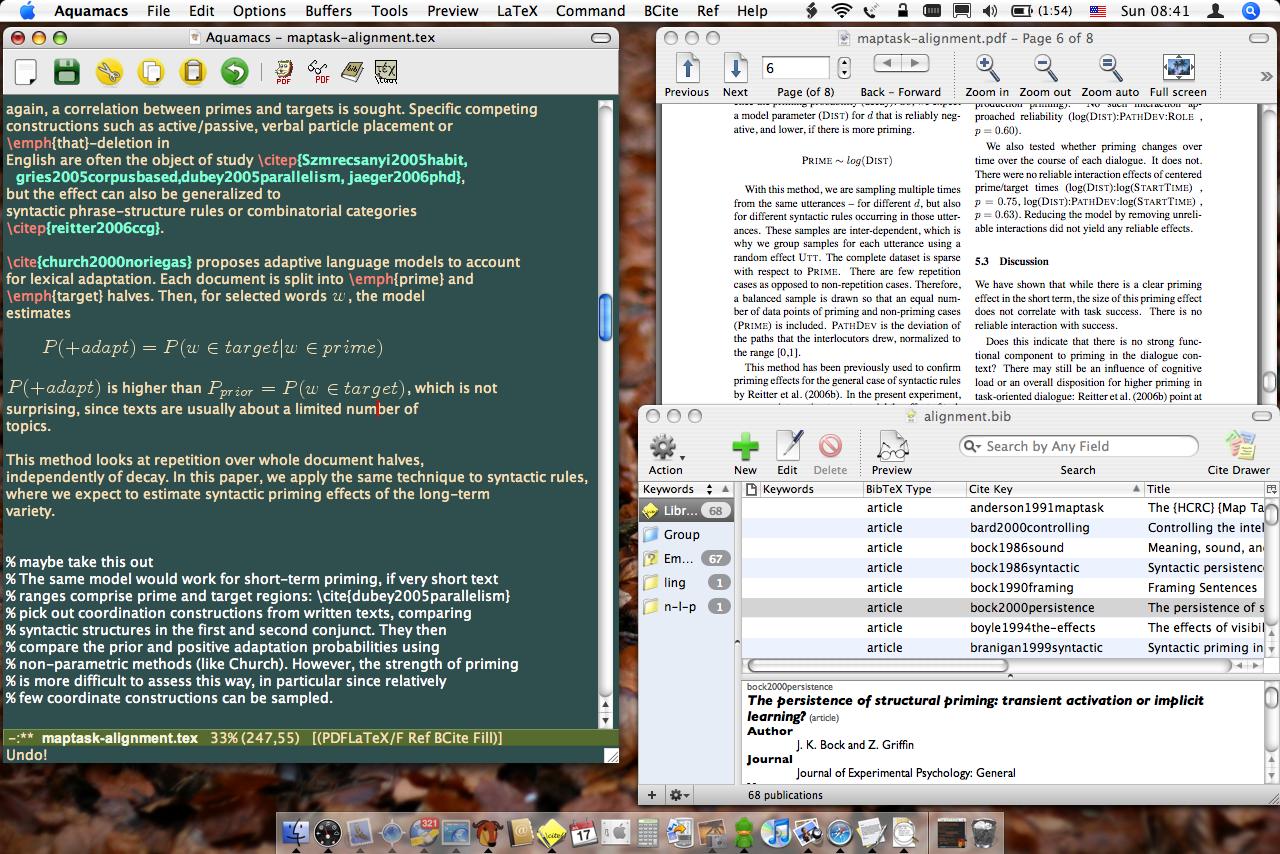
\includegraphics[width=5in]{aquamacs-tex}}
\caption{Aquamacs offers extensive support for \LaTeX\ documents and
  can be combined with viewer applications such as Skim and
  bibliographic databases such as BibDesk.}
\label{aquamacs-tex}
\end{figure}

AUCTeX comes with its own manual, accessible via the LaTeX menu (when in latex mode after loading a .tex file), ``Read the AUCTeX manual''. If you have a question, please consult the manual. If that doesn't work, or you suspect you've found a bug in AUCTeX, please turn to the AUCTeX mailing lists, accessible here: \url{http://www.gnu.org/software/auctex/mailing-lists.html}.

To access the enhanced \LaTeX\ functionality that Aquamacs offers, you will need to install a LaTeX system. We recommend to install the \emph{MacTeX distribution}, available at \url{http://www.tug.org/mactex/}. Alternatively, you can install a smaller distribution provided by Gerben Wierda (\url{http://www.rna.nl/tex.html}. Both install packages are complete and user-friendly. (While you can obtain \TeX\ from other sources, the binary distributions are particularly well supported in Aquamacs.)

Note that AUCTeX, as it comes with Aquamacs, is configured to compile documents directly to PDF, a standard on the Mac. If you prefer to produce DVI and Postscript documents with LaTeX, switch off PDF Mode in Command / TeXing Options.



\subsubsection{Skim: A   \LaTeX\ Previewer}

When editing \LaTeX files, you will often need to view the compiled results. Apple's Preview.app can view PDF files. But for regular use you may prefer a program like \emph{Skim} which has features specifically supporting \LaTeX editing.  Skim is available here:  \url{http://skim-app.sourceforge.net/} .  Skim can automatically reload PDFs every time they are recompiled. It also includes a configuration preset to allow it to jump back and forth between Aquamacs and Skim, showing the documents at the corrsponding locations.  An up-to-date LaTeX distribution such as MacTeX 2009 is required to use the ``SyncTeX'' feature.

Clicking on a position in the PDF file in Skim while holding the
Command and Shift keys causes Aquamacs to move your cursor to the
corresponding point in the underlying source file, opening it if
necessary. To enable Skim with SyncTeX, enable Aquamacs in Skim's
Preferences dialog.  Aquamacs does not need to be configured further
-- it should recognize Skim when it is running (you need to start it
yourself).

If you want to be able to  start Skim  from inside Aquamacs, do the following.

  Having opened a Latex buffer in Aquamacs, go
  ``Menu$>$Latex$>$Customize Auctex'' and then click on "Extend this Menu."
  Then, once more, go ``Menu$>$Latex$>$Cust\-omize Auctex.'' In the list of
  items you see now, drag the mouse to "Tex Command," in the list you
  see then, drag it to "Tex View", and in the list which finally
  opens, click on "Tex View Program Selection." You now have a
  customization buffer opened. There, you see a line which contains
  the words "output-pdf." In the line below that line, you see the
  word "Viewer." To the right of it, there is a button "Value Menu."
  Click on it, and choose "Skim" in the list that pops up.

Finally, before you close the customization buffer, do not forget to click on the button "State" and, in the list then popping up, to click on "Save for Further Sessions". That's all.

Now you can use the view icon in the toolbar, or the key combination
C-c C-v, or ``Menu$>$Command$>$View'' to open Skim with your pdf-output file.

Furthermore, things are configured so that these three ways to call
Skim also yield syncing from source to pdf-output. Syncing from source
to pdf-output can also be obtained by clicking on a position in
your source-file while holding the Command and Shift keys.

(If you had not rejected Apple's default in the installation of Leopard or Snow Leopard to put X11 on your system, you may also consider to choose xdvi for "output-dvi.")


% Older utilities that preceeded Skim were  \TeX niscope and PDFView.  They do not work out-of-the-box with Aquamacs. Using the ``Pdfsync'' package works.


% \subsection{Lisp Support}

% Lisp programmers will appreciate the Superior Lisp Interaction Mode for Emacs, SLIME.  This is available from the Aquamacs website as a convenient point-and-click installer package, which will result in fully integrated Lisp experience.


% \subsection{Java Support}

% Java programmers should install the JDEE point-and-click installer package, available from the Aquamacs website (\url{http://aquamacs.org/download.shtml}).


\subsection{Command Line Tools}

Aquamacs can install command line tools.  Run M-x aquamacs-install-command-line-tool, or choose \emph{Install Command Line Tools} from the Tools menu.
The following commands will be made available from a terminal running the system's default login shell:

\begin{itemize}
\item {\tt aquamacs}: This tool will start up a new Aquamacs or run an existing one.  (If multiple Aquamacs.app application bundles are present in the system, unexpected behavior may occur.  This is a OSX limitation.)   You may give arguments to the tool and use it as {\tt EDITOR} setting.
\item {\tt emacsclient}: This is a tool standard to every GNU Emacs distribution.  It will open a file or execute arbitrary commands in a running Emacs/Aquamacs instance.  (Aquamacs automatically starts the associated server so that you do not need to call M-x server-start.)
\item {\tt emacs}: This tool is installed only if direct install is possible by Aquamacs into /usr/local/bin, on Mac OSX 10.11 or later.   Emacs will start up vanilla mode Aquamacs directly in the text terminal, with no Aquamacs customizations, emulating GNU Emacs.  This allows you to run a late-version Emacs with your system, without the need for installing another package.
\end{itemize}


\subsection{Vanilla Emacs Mode}

Aquamacs may be run in \emph{vanilla Emacs mode}.  This will disable most Aquamacs customizations and prevent loading of included packages.
Aquamacs will be most similar to GNU Emacs.   The mode is intended primarily for terminal use.

To enable the mode, start the Aquamacs process from a terminal, with the {\tt --no-site-file} parameter.

The mode is also enabled by the command line tool {\tt emacs}.



\section{Requirements}
Aquamacs requires Mac OS X 10.6 or later.  The downloadable Aquamacs runs on all modern Macs with 64-bit capable Intel processors.  Versions for older Macs (32-bit Intel, PPC) may be compiled by the end user.

\section{Extending Aquamacs}

Aquamacs supports Plugins that can be packaged to provide point-and-click installers (via Apple's
PackageMaker). The interface is simple. Adding standard Emacs packages is easy as well.

\emph{The plugin interface should be considered deprecated in favor of the available Emacs package management and online repositories such as ELPA or MELPA.}

\subsection{Plug-in Interface (Deprecated)}

All files named \emph{site-start.el} anywhere in the load-path are loaded at startup, before the user's init files are loaded. For example, such a file may be placed in the user's Library folder, that is in \\  {\ttfile \~/Library/Application~Support/Aquamacs~Emacs/myPlugin}.

 The load-path is automatically extended to cover all subdirectories in standard paths (see Section \ref {standardpaths}).

If a plug-in needs to execute code earlier in the initialization phase, that is, before any Aquamacs- specific code is executed (but after Emacs initilization code has been executed), this code can be provided in a file \emph{site-prestart.el} anywhere in the load-path.

Info files (M-x info) can be provided in a directory called {\ttfile info} inside the plugin directory. Aquamacs will automatically add this path to `Info-default-directory-list'. Plugins should provide a {\ttfile dir} file inside the {\ttfile info} directory containing an overview (see the Emacs documentation for `info').

Note that plug-ins should not make any assumptions about whether a frame exists or is visible.


\subsection{Load Path}

Aquamacs is able to find configuration files and Emacs packages
from any of the following standard locations (load-path) in Library folders.
\label{standardpaths}

\begin{itemize}
  \item  {\ttfile /Library/Application~Support/Aquamacs~Emacs/}
  \item  {\ttfile /Library/Preferences/Aquamacs~Emacs/ }
\end{itemize}
The following paths are available in the load-path for individual preference settings. \emph{They should
not be used if you distribute a point-and-click installer package.}
\begin{itemize}
  \item  {\ttfile \~/Library/Application~Support/Aquamacs~Emacs/}
  \item  {\ttfile \~/Library/Preferences/Aquamacs~Emacs/ }
\end{itemize}


All subsequent directories are added recursively, so Aquamacs will
find any path that starts below. Type {\tt C-h v load-path} for more
information.\footnote{The following paths are loaded for backward
  compatibility reasons:
    \begin{itemize}
\item  {\ttfile /Library/Application~Support/Emacs/}
\item  {\ttfile /Library/Preferences/Emacs/ }
\item {\ttfile \~/Library/Preferences/Emacs/ }
\item {\ttfile \~/Library/Preferences/Emacs/ }
    \end{itemize}
. Do not use these paths.}\\



\subsection{Disabling a plug-in or a load-path}

If an (emtpy) file named \emph{.nosearch} exists in a specific path, Aquamacs does not load any \emph
{site-start} and \emph{site-prestart} source files in this or descending paths and does not add that or
subsequent paths to the load-path.



\subsection{Startup files}
In short, most settings are stored in these files:

\begin{itemize}
\item  {\tt \~/.emacs}
\item  {\tt \~/Library/Preferences/Aquamacs Emacs/Preferences.el}
\item  {\tt \~/Library/Preferences/Aquamacs Emacs/customizations.el}

  [Automatically written when you "Save Options"]
\end{itemize}

There are further source files that will be loaded.  So, the complete answer is as follows.

At startup, Aquamacs will load this file:
\begin{itemize}
  \item {\tt \~/.emacs}
\end{itemize}

At startup, by default it will load the following files at startup:

\begin{itemize}
   \item {\tt \~/Library/Preferences/Aquamacs Emacs/customizations.el}
   \item {\tt /Library/Application Support/Emacs/Preferences.el}
[deprecated: don't use!]
   \item {\tt /Library/Application Support/Aquamacs Emacs/Preferences.el}
   \item {\tt \~/Library/Application Support/Emacs/Preferences.el}
  [deprecated: don't use!]
   \item {\tt \~/Library/Application Support/Aquamacs Emacs/Preferences.el}
\end{itemize}

The location of the first customizations file is given by the `custom-file' variable.

Aquamacs will also automatically load all files names {\tt site-start.el} in the load path list, which includes the above paths.

Note that Emacs (including Aquamacs) will preferentially load a {\tt foo.elc} file if present, in lieu of a {\tt foo.el} file, even if the {\tt .el} file is newer.

To trouble-shoot your own customizations, first start Aquamacs "without customizations", which you can do via a function found
in the menu "Help/Diagnose and Report Bug".


\subsection{Changing Aquamacs source files}

If you'd like to tinker with the Emacs lisp source files that come with Aquamacs, you can do so quite easily. When defining a new function or, more generally, to evaluate an expression, C-x C-e is your friend.

However, you may notice that some of your changes aren't active after you've saved your work (into the Aquamacs application bundle) and restart. That is because some of the code is precompiled into the Aquamacs binary and not loaded from the source (or .elc / .el.gz) files. To alleviate that problem, create a
file\\
{\ttfile \~/Library/Application~Support/Aquamacs~Emacs/site-prestart.el} \\ with the following content:


\texttt{(setq aquamacs-reload-preloaded-files t)}

This will cause to re-read the otherwise preloaded files from disk.

\section{Getting Help}

There are many options for getting help with Aquamacs.

From within Aquamacs, you can access user documentation from the menu or from specific key combinations.  This manual is available from the Help menu, as is a very complete Emacs documentation, the \emph{Emacs Manual}.  To extend Emacs using the built-in programming language Emacs Lisp, refer to the \emph{Emacs Lisp Reference}, which is also available from the Help menu.  (The latter can be used via the Mac's convenient Help Books, or via Emacs' powerful Info interface.)

Emacs is self-documenting.  The Help menu (under \emph{Describe}) contains documentation for every function available to the user.  You can reach these functions easily: {\tt C-h k} (plus key/menu entry) brings up help for any key or menu binding; {\tt C-h f} (plus function name) gives help for an elisp function; autocompletion support is available with (tab); and {\tt C-h a} brings up apropos, a search function.

For help from other Aquamacs/Emacs users, the best place to begin is the OS X Emacs mailing list. The searchable list archives are located at \url{http://dir.gmane.org/gmane.emacs.macintosh.osx}. For more information on subscribing to the list, see \url{http://email.esm.psu.edu/mailman/listinfo/macosx-emacs}.  Another option for general Emacs help is the gnu.emacs.help newsgroup.

Remember: almost every question has been asked before.  Google will give you an instant answer, provided you know the right keywords.

Apart from answering questions at the OS X Emacs mailing list, you can also file bug reports on Aquamacs. Use the ``Send Bug Report'' function in the Help / Diagnose and Report Bug menu.  The same menu has a function to restart Aquamacs without any of your customizations -- please use this function to ensure that it is really a bug in Aquamacs that you are seeing.  (Your settings may be flawless, but even so we'd like to know which ones will cause the bug to show up!)

In addition to requesting help, you can also offer it in these mailing lists. \emph{Please note that in case we have helped you with a configuration problem on the mailing list, we may ask you to write a little note in the Aquamacs Wiki so others can benefit, too.} Remember: Aquamacs is an Open Source community project!

\section{Aquamacs Lives From Your Donations}

Aquamacs Emacs is a project that depends on your support. The project
has no other source of substantial income: the application is free,
the downloads are free.

Free software is developed because programmers love their work. Donations will never remunerate them financially as a job in the software industry would. But every donation is a recognition of the programmer's hard work, and the bigger ones actually help paying some bills.

If you would like to say ``thank you'', or if you would like to see
the project developed further, \emph{please make a donation.}

\url{http://aquamacs.org/donate}


\section {Contribute to Aquamacs}

If you'd like to join us in working on Aquamacs, download the source
code from Git and take a look. Do ask if you have questions! When you
have a patch or a less specific suggestion for improvements, send it
to the development mailing list.

We're a very open team. Everyone is allowed to suggest modifications
to every piece of code. There is no ``ownership'' of code, so please
join us to make Aquamacs even better!


\section{Authors and Acknowledgments}

Who's behind Aquamacs?

It's a free software project, and naturally, Aquamacs could not exist
without the help of developers, designers, writers and users. The
following people have contributed code, bug reports and ideas to the
Aquamacs project at one point of the other.\footnote{We apologize for not being able to list everyone.  If you feel that someone should be mentioned, please e-mail us.}

Aquamacs development was led from 2005 to 2019 by David Reitter, a German-American computer scientist and cognitive scientist.

Throughout this time, many contributions in form of bug reports and fixes were provided by Konrad Podczeck, Nathaniel Cunningham, Jos�  Figueroa-O'Farrill, Jean-Christophe Helary, and other regular users.  Win Treese is release manager for Aquamacs starting with 3.6.

Kevin Walzer co-founded the Aquamacs project and wrote the first manual. Aquamacs contains icon artwork by Adrian Chromenko, Jessica Walker (Aquamacs 2.0/3.0 application icon) and David Reitter,
Jasper Hauser, and the Nuovext Project.  The Aquamacs website was designed by Ted Roden.

We would also like to acknowledge the contributions of the many authors
whose source code and hints on public forums have already been
integrated into the build.  They are too numerous to mention here.

Aquamacs is based on GNU Emacs, which is the work of Richard Stallman and many other developers, in particular Andrew Choi (original GNU Emacs-to-MacOS and OSX ports), Steven Tamm, Alan Third, Mitsuharu Yamamoto, Adrian Robert.  Aquamacs also could not exist without the latest code contribtions to GNU Emacs (now lead by Stefan Monnier) and to its Mac/OSX/Nextstep ports ( Jan dj\"arv, Yamamoto Mitsuharu, and others). We also would like to acknowledge the work of the many authors of the major modes included.

Last but not least, Aquamacs exists because of the dedication of
its users, who donate money, report bugs and help us fix them.

\section {Nightly Development Builds}

Ready to install, the Aquamacs project offers nightly built binary
packages that contain the latest in Aquamacs development. These builds
are not considered ``stable'', but experimental.

See \url{http://aquamacs.org/nightlies.shtml} for downloads.


\section {Obtaining the Source Code}

You may download the source code for each release of Aquamacs, or
download the source of the current development version from
\url{http://aquamacs.org/development.shtml}.  You need Git (\url{http://git-scm.com}) in order to download it.

The author offers  to provide you with the source code for a time period of
at least three years from the date of release. Source code should be
obtained from the aforementioned Git repository or,
if this is impossible, by written request from the author.

\section {Licenses}

Aquamacs: the Emacs distribution, (c) 2005--2019 by Free Software
Foundation, Inc., and by David Reitter. Aquamacs is licensed under the
terms of the GNU General Public License, either Version 3, or (at your
option) any later version.

For details of
this license, type C-h C-c in Aquamacs (Help: Copying Conditions) or
visit \url{http://www.fsf.org/licensing/licenses/gpl.html}. The
Aquamacs documentation is licensed under the terms of the GNU Free
Documentation License. For details of this license, please see
\url{http://www.gnu.org/copyleft/fdl.html#SEC1}.

The license does not apply to the toolbar icons contained in the
Aquamacs .app bundle. They may be used and redistributed within
Aquamacs, but not separately or in another application. Some of the
icons may be redistributed, however - see the COPYING file in the etc/images
directory in the Aquamacs .app bundle or in the source code.

The Aquamacs binary distribution includes compiled versions of the following libraries, which are distributed under the specified licenses:

\begin{itemize}
\item libffi: \url{https://sourceware.org/libffi/}, distributed under the following license:
  \begin{quote}
libffi - Copyright (c) 1996-2014  Anthony Green, Red Hat, Inc and others.
See source files for details.

Permission is hereby granted, free of charge, to any person obtaining
a copy of this software and associated documentation files (the
``Software''), to deal in the Software without restriction, including
without limitation the rights to use, copy, modify, merge, publish,
distribute, sublicense, and/or sell copies of the Software, and to
permit persons to whom the Software is furnished to do so, subject to
the following conditions:

The above copyright notice and this permission notice shall be
included in all copies or substantial portions of the Software.

THE SOFTWARE IS PROVIDED ``AS IS'', WITHOUT WARRANTY OF ANY KIND,
EXPRESS OR IMPLIED, INCLUDING BUT NOT LIMITED TO THE WARRANTIES OF
MERCHANTABILITY, FITNESS FOR A PARTICULAR PURPOSE AND NONINFRINGEMENT.
IN NO EVENT SHALL THE AUTHORS OR COPYRIGHT HOLDERS BE LIABLE FOR ANY
CLAIM, DAMAGES OR OTHER LIABILITY, WHETHER IN AN ACTION OF CONTRACT,
TORT OR OTHERWISE, ARISING FROM, OUT OF OR IN CONNECTION WITH THE
SOFTWARE OR THE USE OR OTHER DEALINGS IN THE SOFTWARE.
  \end{quote}

\item GMP: \url{https://gmplib.org}, distributed under the  GNU LGPL v3 and GNU GPL v2.

\item GnuTLS: \url{https://gnutls.org/}, distributed under the GNU LGPLv2.1+.

\item Nettle (a low-level cryptographic library): \url{https://www.lysator.liu.se/~nisse/nettle/}, distributed under the GNU LGPLv3. This is also the source for the bundled Hogweed library.

\item p11-kit: \url{https://p11-glue.github.io/p11-glue/p11-kit.html}, distributed under the following license:
  \begin{verbatim}
/*
 * Copyright (c) 2011, Collabora Ltd.
 *
 * Redistribution and use in source and binary forms, with or without
 * modification, are permitted provided that the following conditions
 * are met:
 *
 *     * Redistributions of source code must retain the above
 *       copyright notice, this list of conditions and the
 *       following disclaimer.
 *     * Redistributions in binary form must reproduce the
 *       above copyright notice, this list of conditions and
 *       the following disclaimer in the documentation and/or
 *       other materials provided with the distribution.
 *     * The names of contributors to this software may not be
 *       used to endorse or promote products derived from this
 *       software without specific prior written permission.
 *
 * THIS SOFTWARE IS PROVIDED BY THE COPYRIGHT HOLDERS AND CONTRIBUTORS
 * "AS IS" AND ANY EXPRESS OR IMPLIED WARRANTIES, INCLUDING, BUT NOT
 * LIMITED TO, THE IMPLIED WARRANTIES OF MERCHANTABILITY AND FITNESS
 * FOR A PARTICULAR PURPOSE ARE DISCLAIMED. IN NO EVENT SHALL THE
 * COPYRIGHT OWNER OR CONTRIBUTORS BE LIABLE FOR ANY DIRECT, INDIRECT,
 * INCIDENTAL, SPECIAL, EXEMPLARY, OR CONSEQUENTIAL DAMAGES (INCLUDING,
 * BUT NOT LIMITED TO, PROCUREMENT OF SUBSTITUTE GOODS OR SERVICES; LOSS
 * OF USE, DATA, OR PROFITS; OR BUSINESS INTERRUPTION) HOWEVER CAUSED
 * AND ON ANY THEORY OF LIABILITY, WHETHER IN CONTRACT, STRICT LIABILITY,
 * OR TORT (INCLUDING NEGLIGENCE OR OTHERWISE) ARISING IN ANY WAY OUT OF
 * THE USE OF THIS SOFTWARE, EVEN IF ADVISED OF THE POSSIBILITY OF SUCH
 * DAMAGE.
 *
 * Author: Stef Walter <stefw@collabora.co.uk>
 */
\end{verbatim}

\item libtasn1: \url{https://www.gnu.org/software/libtasn1}, distributed under the  GNU Lesser General Public License version 2.1 or later.n

\item libunistring: \url{https://www.gnu.org/software/libunistring/}, distributed under the GNU Lesser General Public License (LGPL).

\item libxml2: \url{http://www.xmlsoft.org/}, distributed under the MIT License.
\end{itemize}

% Change log is too long to be included here.
\begin{htmlonly}
\section{Aquamacs Emacs: What's New in This Release}

\subsection{Changes--- 3.5}
\begin{rawhtml}
<a name="changelog-top"></a>
\end{rawhtml}
\textbf{Thank you to all supporters.  To donate to the project, go to: \url{http://aquamacs.org/donations.shtml}.}
\vskip2em
\begin{itemize}
\item Fixed a compatibility issue with macOS Mojave.
\item Aquamacs is now compiled and distributed with a copy of the gnutls library to enable secure web connections. The version in this distribution is 3.6.8. Only the shared library  and its library dependencies are included. This was done because Emacs has removed support for using the openssl command line tool shipped with Mac OS X. Code for building the libraries contributed by Win Treese. License information for these libraries is included the manual.
\item In order to provide compatibility with gnutls, the oldest  supported version of Mac OS X is now El Capitan (10.11).

\item This version also bundles the binary shared library for the libxml2 library (version 2.9.9).
\item ESS has been updated to version 18.10.2.  See here for all new features: \url{http://ess.r-project.org/Manual/ess.html#New-features}.

\item Known bug (MacOS Mojave): menus may require a double click to open with
  the mouse.  When this happen, go to System Preferences, Security\&Privacy, Accessibility, and allow Aquamacs to ``control your computer''. This merely enables Aquamacs to process some UI events.

\item Bug fix: a rare condition (when Tabs are not in used) could occur where frames will be unresponsive to user input.   Reported by Lewis Hyatt.

\item Bug fix: Color lists were unavailable on late MacOS versions.  Reported by Max Arnold.

\end{itemize}


\subsection{Changes--- 3.4}
\begin{itemize}
\item Aquamacs no longer sets colors in `default-frame-alist' as a default to
  make customization with themes easier.
\item `aquamacs-styles' has been removed.  (Deprecated in version 1.6.)
\item Printing at 100\% uses a reasonable font size.  Also, printing respects scaled font size again.
Reported by Matthew Cornell.
\item Scrolling with the mouse has been adjusted (less jerky, but progressive).  Reported by Sam Coskey and David Poole;
  code contribution by Jamie Taylor.
\item Bugs in version checking fixed (redirecting Wifi landing pages; menu item use).
\item {\tt --debug-init} works again as a command-line argument.  Reported by Bob Harper.
\item AUCTeX has been updated to version 12.1 (from version 11.89).  This improves command completion and fixes bugs.  See here for further changes:  \url{http://www.gnu.org/software/auctex/manual/auctex/Changes.html}.
  \item ESS has been updated to version 17.11.  See here for all new features: \url{http://ess.r-project.org/Manual/ess.html#New-features}.
\item OneOnOne package (by Drew Adams) updated.
\end{itemize}


\subsection{Changes--- 3.3}
\vskip2em
\begin{itemize}
\item Aquamacs is now based on Emacs 25.1.  A selection of new, user-visible features is:
\begin{itemize}
\item Improved undo (for deletion of characters).
\item Improved Unicode support (see NEWS for details)
\item Search functions (Command-F / C-s) are now more flexible in matching characters.  Configure `search-default-mode' to turn this off.
\item Tramp supports afp for Apple File Servers.
\item The new command 'vc-region-history' shows the log+diff of the active region.
\item 'compare-windows' now compares text with the most recently selected window instead of the next window.
\item C-h k KEY will now tell you not only what this key command does, but also in which keymap it is bound to the command.  This is useful especially in Aquamacs if you would like to override a key binding.
\item 'setq' and 'setf' must now be called with an even number of arguments.
\item (Multicolor fonts remain supported on Aquamacs.)
\item For further details, and a list of all changes in Emacs 25.1, please refert to etc/NEWS at \url{http://www.gnu.org/software/emacs/NEWS.25.1} (once released).
\end{itemize}
\item MELPA is now available as a source of packages to install.  The Options menu has a \emph{Manage Emacs Packages} command.
\item The \emph{Copy Formatted} function (formerly \emph{Copy Styled as HTML}) is now compatible with any Mac application that can insert formatted documents, including Apple's Keynote and Pages, as well as MS Word.  The \emph{Copy as PDF} function exports a small PDF clipping with the region that is widely usable, including in MS Powerpoint.
\item The color for printing text is now always black unless fontification chooses a different color.  If a dark background is used, colors for black-on-white printing are always darkened.  (Configure with `htmlize-white-background'.)

\item Aquamacs is again usable from a text terminal (start with -nw), with backspace and C-h being recognized properly.
\item The commandline tools installation function has been updated for Mac OSX ``El Capitan''.
Reported by Steve Ward.
\item A script called \emph{emacs} is provided that will start Aquamacs on the command line (in a text terminal) in a mode that starts up rapidly and provides UI compatibility with GNU Emacs (rather than Aquamacs).  This is installed by the command \emph{Install Command Line Tools} (Tools menu, or M-x aquamacs-install-command-line-tool).  The emacs script is non-relocatable and needs to remain in the Aquamacs bundle.  You may link to it.
\item filladapt mode is no longer automatically activated, as it hinders compatibility with some modes.  Emacs now provides improved filling on its own, see \url{https://www.gnu.org/software/emacs/manual/html_node/emacs/Adaptive-Fill.html}.  Requested by Win Treese.   Filladapt continues to be available to users who need it.  It can be loaded by adding {\tt (require 'filladapt)} to the {\tt Preferences.el} file.
\item Apple Emoji symbols can now be displayed.

\item Cc-mode is about 30\% faster in displaying code and scrolling.
\item Swift-mode (version 0.5.0-snapshot) provided for editing Swift files.
%  backed out.  \item Flycheck included (version 0.25.1).  Users typically need to install external syntax checkers.  See the manual: \url{http://www.flycheck.org/manual/latest/index.html}.
\item Python-mode updated to version 6.2.2 (was: 6.1.3).  For what's new, see \url{https://gitlab.com/python-mode-devs/python-mode/blob/master/NEWS}.
\item Emacs Speaks Statistics (ESS) has been upgraded to 16.04 (was: 14.09).  The change brings automatic code formatting and improved indentation, among other features. See here for all new features: \url{http://ess.r-project.org/Manual/ess.html#New-features}
\item AUCTeX has been updated to version 11.89 (from version 11.88).  Notably, there is now a ``Compile and View'' function (bound to C-c C-A).  See here for further changes:  \url{http://www.gnu.org/software/auctex/manual/auctex/Changes.html}.

\item Prevent a hang condition or crash during automatic startup after reboot or login.
Patch by Anders Lindgren.
\item Errors in default frame settings are caught and properly reported at startup now.
Reported by Pete Siemsen.
\item Prevent a crash when viewing a LaTeX PDF file in Skim.
\item Prevent crashes when, after display of save or print panels, certain keys (enter) were pressed.
\item Improve maximization behavior of frames (Option-click into green window button).
Reported by Idar Tollefsen.

\end{itemize}
\subsection{Changes--- 3.2}
\begin{itemize}
\item On OS X 10.10 ``Yosemite'', clicks on toolbar icons could cause Aquamacs (as well as GNU Emacs 24.4) to become unresponsive.  Until Apple releases an improved version of the operating system, Aquamacs provides a workaround.
\item Color dragging out of the color palette (and other drag\&drop actions) right after startup now works reliably.
\item Color dragging to set colors of the fringes in a window works again.
\item The size of LaTeX previews on Retina displays has been corrected.  For convenience, Aquamacs will no longer ask whether to ``cache the preamble'' (who knows what that entails anyway?).
\item AUCTeX has been updated to version 11.88 (from version 11.87). See here for what's new: \url{http://www.gnu.org/software/auctex/manual/auctex/Changes.html}.
\end{itemize}
\subsection{Changes--- 3.1a}
\begin{itemize}
\item Command-Shift-Left/Right now select the text from point to the left or right side of the line, as they did in Aquamacs 2.
Reported by Daniel Stegm\"uller.
\item The order of menu items in the Options/Line Wrapping submenu has been restored.
Reported by Gracjan Polak.
\item Isearch using the Mac key bindings (A-f, A-g) has seen some improvements.  A-g will now highlight all other search results (just like regular isearch), and it will continue a regexp isearch (started with C-u A-f).  Because you remain in `isearch-mode' after a A-g, additional simple keys will just extend the search string.  (You may, as before, do other things like insert text clippings with A-v.)
\item During Isearch started with A-f or A-g, you may now use the Enter (RET) key to advance to the next location, and S-RET to go back to the previous one (same bindings as A-g and A-S-g).  This is in accordance with search functions in other Mac applications.  Traditional Emacs behavior of isearch when started with C-s is not affected.
Suggested by Jeremy Cole.
\item Cursor motion with arrow keys will follow the
visual order of characters on the screen: \emph{left} always moves to the
left, \emph{right} always moves to the right, disregarding the surrounding
bidirectional context.  You may change this setting with the customization variable `visual-order-cursor-movement'.
\item Aquamacs is now based on Emacs 24.4.  Please see etc/NEWS for detailed information.  Some more important, user-visible changes are:
\begin{itemize}
\item Frames and windows now resize smoothly, pixel by pixel.
\item In keymaps where SPC scrolls forward, S-SPC now scrolls backward.
This affects View mode, etc.
\item The cursor stops blinking after 10 blinks (by default) on X and Nextstep.
You can change the default by customizing `blink-cursor-blinks'.
\item `electric-indent-mode' is now enabled by default.
Typing RET reindents the current line and indents the new line.
C-j inserts a newline but does not indent.  In some programming modes,
additional characters are electric (eg `\{').
\item The behavior of C-x TAB (`indent-rigidly') has changed.
When invoked without a prefix argument, it now activates a transient
mode in which typing left, right, S-left, and S-right adjusts
the text indentation in the region.  Typing any other key resumes
normal editing behavior.
\item New command C-x SPC (`rectangle-mark-mode') makes a rectangular region.
Most commands are still unaware of it, but kill/yank do work on the rectangle.
\end{itemize}
\item Package-specific information is now stored in {\textasciitilde{}}/Library/Preferences/Aquamacs Emacs/Packages.  Files are automatically moved to the new location so that correctly implemented packages should not be affected.  (Switching to a previous Aquamacs version, however, will cause some settings to be lost.)
\item Tramp reliability improved.
Reported by Steve Bellan.
\item `ams-tex-mode' is functional again.
Reported by Albert Fisher.
\item Switching buffers when tabbar-mode (``Show Tabs'') is off and one-buffer-one-frame-mode (``Show Buffers in New Frames'') no longer produces an error message in certain situations.
Reported by Bob Berwick.
\item Dragging and dropping colors from the color selection panel now works more reliably.
Reported by Konrad Podczeck.
\item ESS mode was updated to version 14.09. See here for new features: \url{http://ess.r-project.org/Manual/ess.html#New-features}
\item Markdown-mode 2.0 is now provided with a default configuration of its faces, which no longer hides markup.
\item Version 3.1a only: an incompatibility with older OS X versions (pre-10.9) and the use of secondary displays was resolved.
Reported by Erik Marklund.
\item Version 3.1a only: a warning indicating a failure to create a file in the Library folder (in new installations) has been resolved.
Reported by `xenzo' and Torsten M\"ahne.
\end{itemize}

\subsection{Changes--- 3.0}


\begin{itemize}
\item This Aquamacs is based on Emacs 24. Highlights:
\begin{itemize}
\item A major addition to Emacs 24 is its package managing system.  (Start with M-x list-packages.  Re-installing included packages is not recommended.)
\item There is a new word count function (see Aquamacs Edit menu).
\item Right-to-left text (Arabic, Persian, Hebrew) is well supported now even when mixed with left-to-right text.
\item Completion has been improved (e.g., it is connected to the CEDET Semantic library.  When enabled, you can use M-Tab to complete symbols in C mode, for instance.)
\item Please refer to \url{http://www.gnu.org/software/emacs/news/} for a list of changes in GNU Emacs 24.
\end{itemize}
\item Aquamacs 3.x is distributed as a binary for 64-bit Intel Macs only.  If you would like to run Aquamacs on a 32-bit Mac, or a PowerPC based Mac, you may still build it yourself from source, or use Aquamacs 2.5.
\item High-resolution retina screens are better supported by the `preview' function in LaTeX mode.  Previews are rendered in a size adjusted to the font used to edit the document.
\item New, high-resolution icons appear in the toolbar (for LaTeX); standard visual effects and animations are used for new frames.
\item `mouse-drag-copy-region' is enabled (non-nil), which maintain behavior similar to that of the previous Aquamacs and Emacs versions.  Selecting some text with the mouse will add it to the kill-ring, so that users may insert it with C-y.
\item The region is no longer extended when dragging the mouse while holding the Shift key, because the `mouse-sel' package is now obsolete in Emacs 24.  Users can, for the time being, bring back the functionality by adding the following to their {\tt Preferences.el} file:
\begin{verbatim}
(require 'mouse-sel)
(global-set-key (vector '(shift down-mouse-1)) 'mouse-extend)
\end{verbatim}
\item Smart spacing no longer affects text yanked with mouse-2 (Command-mouse click), for the the time being.  To get this added convenience, {\tt (global-set-key (vector `(mouse-2)) 'mouse-yank-at-click)} may be used.
These hints suggested by Konrad Podczeck.
\item Abbreviations are, by default, persistant: they are saved upon quitting Aquamacs.  Configure `save-abbrevs' to change this default.
\item {\bf paredit-mode} is included (version 23), which provides operations that, in Lisp, preserve the integrity of the syntax trees (i.e., keep/delete s-expressions as a whole).  See here for more information: \url{http://www.emacswiki.org/emacs/ParEdit}, and here for an informative screencast: \url{http://emacsrocks.com/e14.html}.
Written by Taylor R. Campbell.
\item {\bf dart-mode} (version 0.9) included.  Written by Nathan Weizenbaum. File endings: {\tt .dart}.
\item {\bf markdown-mode} (version 2.0) included.  Written by Jason R. Blevins. File endings: {\tt .md}.
\item {\bf python-mode} updated to version 6.1.3 (pre-release 2014-01-19).  Comes with a streamlined menu and many detailed improvements, but drops Pymacs integration.  Aquamacs will bring back Ropemacs and Pymacs in a future version.  See here for changes: \url{https://launchpad.net/python-mode/+announcements}
\item {\bf Emacs Speaks Statistics (ESS)} updated to version 13.09-1. See here for changes: \url{http://ess.r-project.org/Manual/news.html}
\end{itemize}
\subsection{Changes--- 2.x}

\begin{itemize}
\item The default directory for buffers is the home directory in OS X 10.9 ``Mavericks'' as in previous OS X versions.
Reported by Christopher Stacy.
\item Isearch no longer aborts a search at seemingly random (but rare) times.  Reported by Bill Sacks.
\item Clicking on the Aquamacs dock icon will again create a new buffer or de-minimize a window, as is standard on OS X.
Reported by Guy Gascoigne-Piggford.
\item A certain rare crash when viewing a compiled LaTeX file (and in other situations) has been addressed.  Thanks to all who reported it.
\end{itemize}

\subsection{Changes--- 2.5}

\begin{itemize}

\item Aquamacs is now signed and will now execute with the default GateKeeper settings in OS X 10.8.
\item Full-screen now supports the standard Mac OS X 10.7 ``Lion'' full-screen mode:  The frame takes up the full (main) display and uses its own screen.  Users may switch between screens as usual (mouse swipe or C-left/right, for instance).  The old-style fullscreen mode is still available, however.  To maximize a frame on the current space, allowing other frames on this space, type C-u A-S-Return, or prepend any of the commands that enter fullscreen mode with C-u.
Thanks for research: Sandy Patterson and Daisuke Murase.
\item Retina displays are now supported (high-resolution artwork is included in most cases).  LaTeX Preview mode (AUCTeX) has been modified to show high-resolution previews.  (Technical note: other packages can be updated by providing TIFFs with multiple resolutions, or by generating high-DPI images, setting their DPI meta information correctly, and setting the new `ns-true-dpi-images-filename-string' variable while loading images.)
\item S-tab no longer mapped to C-y (ASCII 25, end of medium). Now properly handled as backtab.  Patch by Gracjan Polak.
\item Aquamacs now provides experimental session persistency:  you can load and save sessions.  Use the new {\em Load Session, Save Session As} menu entries in the {\em File} menu to use these new functions.  Note: Unlike the formerly available functions from the `desktop' package, all frames, windows, tabs, buffers and some customizations are saved.  Buffers not linked to a file, such as those showing processes, will not be restored, and frames may not end up on the same space at this time.  Aquamacs now includes an adapted version of the {\tt revive.el} package by Hirose Yuuji.  We recommend that you do not load a different version of this package yourself.
% , and under Mac OS X 10.7 or later, sessions are reguarily saved and restored in case of unexpected program termination or reboot
% and the new customization variable `revive-desktop-after-launching' to turn the behavior off, or enable automatic session persistency even on pre-Lion operating systems
\item Colors are now displayed in the ``color space'' that is set by the user for the specific display.  A slight change in color shades may be noticed.
Suggested by Juan Jose Garcia Ripoll.
\item Text search (isearch) now works better when using one of the Emulate-Mac-Keyboard-Modes.
Reported by Thomas Strathmann.
\item Frames are now reliably moved inside the current display again when entering the minibuffer (and at other times).
\item Switching applications while Aquamacs is in full-screen mode no longer creates unwanted empty frames.
Reported by Christian H\"o{}ltje, Rory Kirchner and Milan Mitrovi\'c{}.
\item ESS upgraded to 13.05. (Previous version was 5.13 - no joke. The ESS version numbering changed.) See here for changes: \url{http://ess.r-project.org/Manual/ess.html#New-features}
\item AUCTeX upgraded to 11.87. (Previous version was 11.86.) See here for changes: \url{http://www.gnu.org/software/auctex/manual/auctex/Changes.html}
\item Python-mode upgraded to 6.0.8.  (Previous version was 6.0.2.)  See here for changes: \url{https://launchpad.net/python-mode/+announcements}
\item Prolog-mode upgraded to 1.23. (Previous version was 1.22.)  (Added support for XSB.)
\end{itemize}

\subsection{Changes--- 2.4}
\begin{itemize}
\item Added {\it visual-basic-mode}.
Code by Fred White, Dave Love, Randolph Fritz and Vincent Belaiche.
\item Fix crash that could occur during start of Aquamacs (in {\it x\_set\_frame\_parameters})
Reported by Will Morton, Barbara Shirtcliff, Enrico Rinaldi.
\item Support for fullscreen button in windows, available in Mac OS X 10.7 ``Lion''.  As additional keyboard shortcut, Command-Control-F, is available.
\item Improved support for resizing frames in Mac OS X 10.7.
\item Load calculator (M-x calc) correctly even after saving calculator settings.
Reported by Stefan Vollmar.
\item When deleting (killing) a whole line, the beginning space of a following line was deleted in `smart-spacing-mode'.  This is no longer the case.
Reported by James Thurgood and Robert Morelli.
\item When deleting several words in a row (killing them to append them to the kill ring), they are no longer added as run-in words in smart spacing mode.  Spaces are addes where appropriate.
\item Switching to Aquamacs or between spaces has been revised.
\item Drag\&drop into windows showing eshell, shell and other comint-based buffers now inserts the full file name.
Suggested by Jan Marius Hofert.
\item When expanding the load path (e.g., for library files) in directories such as Library/Application~Support/Aquamacs~Emacs, a file called {.nosearch} now prevents Aquamacs from adding the present and subordinate directories.  (The previous {\tt .ignore} file only worked at the topmost level.)
Reported by Nathaniel Cunningham.
\item Fixed issue that could lead to a crash when using Aquamacs as an editor (ODB standard) from certain other applications.
Reported by Kevin Kirkup.
\item Fixed issue where the toolbar could not be permanently hidden or shown using the toolbar context menu.
Reported by Richard Spence.
\item {\tt Python-Mode} has been updated to version 6.0.2.
Suggested by Gilles Lenfant.
\item {\tt Matlab-Mode} has been updated to version 3.3.1.
Suggested by Dennis Rosset.
\end{itemize}


\subsection{Changes--- 2.3}
\begin{itemize}
\item Correct substantial display problems that occured when  the cursor type was set to `box' shape.
Reported by many people (thanks).
\item Display text behind a filled box cursor in the background color.
\item Allow `cursor-type' to be set to (bar . WIDTH) with an arbitrarily large width.
Reported by Konrad Podczeck.
\item Fix insertion of the Euro sign with Option-e under emulate-mac-*-keyboard-mode.
Reported by Viktor Rosenfeld.
\item Updated ESS (Emacs Speaks Statistics) to version 5.13.
\end{itemize}

\subsection{Changes--- 2.2}

\begin{itemize}
\item Improved fullscreen mode: addresses rare display issues (related to scrollbars), crashes after switching back from fullscreen mode, and empty menus during fullscreen mode.  Note that multiple frames may be shown in fullscreen mode (switch with, e.g.,  A-`).
Code by Daisuke Murase and David Reitter.  Suggested by many.

\item  \emph{Improvements to working with Frames and Spaces:}
\begin{itemize}
\item Repeated cycling between frames (forwards with A-`) now cycles through all frames rather than just the two most recent ones.
Suggested by many Aquamacs users.
\item When deleting a frame in one space, Aquamacs no longer switches to another space if there is one (10.6 only).
\item When opening a frame via drag\&drop or the terminal command-line, Aquamacs now shows the frame in the currently active space if `one-buffer-one-frame' or `tabbar-mode' are on (10.6 only).
\item No more unnecessarily space switches away from a new frame created after drag\&drop, Finder or terminal-based opening of files in certain situations.
Patch by Ted Middleton.
\item The menu bar works again after switching away to a space without an Aquamacs frame on it.
\end{itemize}
\item \emph{Spell-checking improvements:}
\begin{itemize}
\item Ability to ignore misspellings on a per-buffer basis, using buffer comments, has been added to the spelling context menu: ``Ignore Spelling \& Comment Buffer''.  Suggested by Konrad Podczeck.
\item ``Check Spelling While Typing'' (`flyspell-mode') is now automatically activated when ``Spellcheck Now'' (`flyspell-buffer' or `flyspell-region') is run with the default OS X spellchecker.  Customize via variable `flyspell-mode-auto-on'.
\end{itemize}
\item Aquamacs starts up faster.
\item New, untitled buffers are now auto-saved regularly, just like buffers visiting files.
Suggested by Andrew Sullivan.
\item Aquamacs can now be used as external editor to ODB-enabled applications such as most FTP clients, Apple XCode 3.x, and other programs in need of an editor.  (Some applications may require changes to recognize Aquamacs--contact their makers to ask for support.)
\item There is a function in the Help / Diagnose menu now to debug one's preferences (init) files such as {\tt Preferences.el} or {\tt .emacs}.  This starts a new Aquamacs process, which, as the one started without customizations using its own menu entry, is no longer dependent on the primary one.
Code by Ze'ev Celementson.
\item The manuals have been unified in order to provide cross-manual keyword search (Help menu).  Also (reported by Joseph van Andel), links to separate manuals (such as Tramp, CC Mode and many others) now work: those manuals are now included as Apple Help variants.
\item Users can now edit all existing user-editable preferences files ({\tt Preferences.el} in various places, and {\tt .emacs}) using a new menu entry in the Help/Diagnose menu.
\item In case Aquamacs crashes, a detailed bug report can usually be sent upon the next program start.
\item The Copy as HTML function (Edit menu) now copies the region with all formatting such that the formatting is preserved in other (Cocoa) applications.
\item Aquamacs can now be configured to not kill a buffer when its last window is deleted through commands such as `close-window' (Command-W).  Set the
new customization open `delete-window-preserve-buffer' to {\tt t} to retain buffers.
Suggested by José M. Figueroa-O'Farrill.
\item When using {\tt emacsclient -t} to connect to a running Aquamacs session from the terminal, entering the minibuffer no longer produces an error.
Reported by Stephen T.
\item When hollow cursors are used, ensure that the glyph underneath the cursor remains visible.
Reported by Marcin Koziej.
\item A rare issue where the wrong images (e.g., a ``redo'' toolbar button in place of a tabbar tab-close button) where displayed, has been addressed.
\item Find-file (C-x C-f) with a file that is already visible in another window now switches to that window again (`one-buffer-one-frame-mode' being on).
Reported by Dan Coe.
\item Cursor movement (up/down) is more precise in terms of horizontal placement.
Reported by Matt Crawford.
\item Improved compatibility of the language-layout specific keyboard emulation modes.
Reported by Santiago Gaviria.
\item Html Helper Mode: Improve recognition/update of time stamps in files.
Patch by Dave Mason.
\item nXhtml Mode is now included (to use, type M-x nxhtml-mode.  Version 2.08 (04/2010).  This also provides \emph{Multiple Major Modes}.
\item Compatibility with Emacs Code Browser has been improved (menus appear correctly, cursor blinks and windows retain selection).
Reported by Martin Sivak.
\item Exporting to a temporary buffer in `org-mode' no longer fails, nor does calling `normal-mode'.
Reported by Jeff Horn and Lawrence Mitchell.
\item AUCTeX now supports Ghostscript 9.01.
Fixed by Denis Rosset.

\end{itemize}

\subsection{Changes--- 2.1}


\begin{itemize}


\item Aquamacs is now optimized further for speed on machines with Intel processors: It starts up faster and also executes lisp faster (up to 50\% in some situations).
\item The ``Line Numbers'' item in the Options/View menu now turns on `global-linum-mode', displaying line numbers to the left of each buffer line.
Suggested by Konrad Podczeck.
\item Copying bug reports and other mail to the pasteboard in order to send them with GMail or another mail program now works reliably.
Reported by Matt Mollison. % AQUAMACS-1.X
\item C-x s (`save-some-buffers') and other functions that ask questions applying to a series of items accept the {\tt !} command again to apply the action to all items (e.g., save all buffers).
Reported by Michael Kohlhase.
\item Users should now experience no more trouble binding the new Aquamacs version to file types with the Finder's ``Open With'' and ``Change all'' functions when earlier versions of Aquamacs are present.  In case of persistent issues, we advise to reset the LaunchServices database with the `lsregister' command as described here:  \url{http://www.macosxhints.com/article.php?story=20071102084155353}
Reported by Arthur Ogus
\item The Spellchecking context menu (flyspell-mode / Check Spelling While Typing) now shows suggested alternatives in the right order.
\item The LaTeX icon in the toolbar changes again when toggling PDF mode.
Reported by Gabriel Cardona and Konrad Podczeck.
\item Jumping to the exact source/PDF position with Skim now works even in multi-file LaTeX projects where files are in different locations.
Reported by Brad Miller and Jeffery Kline.
\item Setting frame position and size in `default-frame-alist' (and elsewhere) now works again.
Reported by Konrad Podczeck.
\item Fixed ``Join Windows'' menu item (was: ``Remove Splits'').
\item PHP-mode has been updated to version 1.5.0.
\item Files opened from the command line or via the Finder will be shown if they are already visible in a tab or in any other window;  unless `Show Buffers in New Frames' (one-buffer-one-frame-mode) is enabled, Aquamacs no longer creates a new frame for those files.  The customization variable `dnd-open-file-other-window'  can be used to control the behavior.
Reported by Mike Pelican.
\item With all frames closed, minimized or on other spaces, Aquamacs now recognizes key commands again.  If the minibuffer is needed, a frame showing an \emph{empty} buffer will appear.  This buffer is always read-only and, unsurprisingly, rather empty.
\item Frames are now cycled in order of their last selection, rather than their creation.  Selecting a frame and deleting it will, for instance, select the previously selected frame.  Cycling with A-` (`next-frame')  will cycle accordingly.
Reported by Konrad Podczeck and David Eyk.
\item Haskell-mode has been updated to version 2.7.0.
Suggested by Johannes Krause.
\item Menu-bar-mode, not supported in Aquamacs, will no longer cause problems for people who try to switch the menu bar off in their customizations.
\item The cursor is now drawn correctly when `line-spacing' is set.
\item Aquamacs no longer hangs in some situations when using `ispell'.
\end{itemize}



\subsection{Changes--- 2.0}


\emph{Aquamacs is now based on Emacs 23 and the Cocoa NextStep port.  There are many changes under the hood associated with this, but also a plethora of visible improvements.  Major ones, and those pertaining to Aquamacs specifically, are listed here.  Further changes can be found in the NEWS file for Emacs 23.}


\textbf{Major User Interface Improvements}


\begin{itemize}
\item Spell-checking now uses the system-wide dictionaries in all the languages supported on OS X.  The standard spelling user interface is available as well as the traditional Emacs `ispell' interface (which also uses the system-wide spelling mechanism).  Configure the use of GNU `aspell' through the `ispell-program-name' variable if desired.

Code by Nathaniel Cunningham.

\item Aquamacs has a new icon in the Dock, designed by graphic designer Jessica Walker (jekawacaneer@gmail.com).

\item The Aquamacs application has been renamed to \emph{Aquamacs.app} (from Aquamacs Emacs.app).

\item Dialogs have been vastly improved: they appear as sheets over the frames where they belong, contain better UI elements (as in the case of the dialog displayed before quitting Aquamacs, which was once called ``dialog from hell'' before receiving a makeover).  The standard Enter, Space and Esc keys (and more) are supported.  ``File Save'' panels also appear as sheets.

\item Toolbars can now be configured through the normal customization panel.  Right-click on the toolbar, use the Options/View menu item (or use M-x ns-tool-bar-customize).  The chosen icons are persistent; toolbar customizations are, however, tied to the toolbars set by modes.  That means that users can chose a different set of icons to display in latex-mode, for instance.
The `ns-tool-bar-display-mode' variable now supports label-only toolbars.  Right-click on the toolbar to change; or use M-x customize or {\tt Preferences.el} to set it to `labels' in order to only show labels.  The former meaning of this value (showing labels and icons) is now `both' (or, usually, nil, the default).

\item Fonts and colors of all (mode-specific) faces can now be configured using the standard font and color panels.  The Options / Appearance menu provides a function to show the font panel, which leads to buttons for foreground and background colors.   We also have a menu item for the color panel separately, from where colors can be dragged\&dropped directly onto any piece of text to customize its face.  Holding down the Option key will, instead, set the face's background color.

\item The printing system has been revised; the standard print and page setup dialogs are used inside the application.  The print dialog now appears more quickly.  (Note: over-long lines will always be wrapped at word boundaries when printing. Clipping or horizontal pagination are not supported at this time.)

\item Line wrapping is now set to Truncate, Wrap, Word Wrap and Line Breaking (auto fill) under \emph{Options / Line Wrapping} for the current buffer.  A \emph{Set as Default} will set it as default for all buffers that have no explicit line wrap setting.  As before, there is also a setting to detect word wrap in text files.  When it is on, Aquamacs detects the wrapping style of text-mode buffers automatically, but prefers word wrapping (see the customization variable `auto-word-wrap-default-function').
{\small Word Wrapping translates to `visual-line-mode' internally now, and the former Aquamacs 1.x mode of the same name now corresponds to a customization variable called `line-move-visual', which is enabled by default.  `Longlines-mode' is obsolete.   Users with manual customizations should adjust their settings.  Fine control can be achieved by customizing `visual-line-mode', `word-wrap', `truncate-lines', and `auto-fill-mode'.}

\end{itemize}



\textbf{Key Bindings}

\begin{itemize}


\item It is now possible to customize behavior of right Option/Alternate, Command and Control modifiers independently of the left ones using new entries in the (renamed) ``Option, Command, Meta keys'' menu (in Options) or the new customization variables named `ns-right-alternate-modifier' (etc).
Patch by Marcin Koziej.

\item Even when the Option modifier keys are set up to be handled by the system (rather than being Meta - see Options - Option Key menu), Option-Arrow and Option-Delete key combinations lead to wordwise operations (they are recognized as Meta).  (Set the new `ns-alternate-meta-special-codes'  to nil to disable.)

\item Note that Word Wrapping (`visual-line-mode') affects the function of the cursor movement keys (arrows, and C-a, C-e, C-p and C-n).  In Aquamacs, this can be easily customized.  The default is as such:
\begin{itemize}
\item In Word Wrapping (visual-line-mode), C-aenp and arrow keys move according to visual lines.
\item Without Word Wrapping (visual-line-mode off), arrow keys move visually, but C-aenp move non-visually according to buffer lines as in Emacs 22 and Aquamacs 1.x.
\end{itemize}
Users may configure this behavior via the (new) `line-move-visual' customization variable.  Set it to \emph{t} for unconditional visual movement of all keys, and \emph{nil} for unconditional logical (buffer) movement of all keys.

\item Keyboard bindings are displayed more consistently in the menus now.  Throughout Aquamacs,  Mac standard key descriptions are used (this may be configured using the variable `ns-use-mac-modifier-symbols').  Users should be aware that manuals and tutorials will often refer to keys such as {\tt C-x} ({\tt \^X} or Control X), and that keys like {\tt M-q} correspond to the chosen Meta key modifier, normally the Option key.

\item Tabs are now available via the A-1..9 (Command-1..9) keybindings.  `Split-window-vertically' is now bound to A-M-2 (Command Option 2), `split-window-horizontally' is A-M-3 (Command Option 3).

\item Command-{\textasciitilde{}} ~now cycles backward to the previously selected frame (`raise-previous-frame').
Patch by Matthew Dempsky.

\item Command-Meta-; now runs `flyspell-buffer', which marks all misspellings in the current buffer.
Patch by Nathaniel Cunningham.

\item Command-PageUp/PageDown now jump to the beginning or end of the buffer, respectively (`beginning-of-buffer', `end-of-buffer').

\item When `osx-key-mode' is switched off, `x-select-enable-clipboard' is restored to its (new) default value, \emph{t}. That means that kill and yank operations (C-w, C-y, mouse text selection and more) are integrated with the Mac pasteboard.  When `osx-key-mode' is on (as is default), everything is as in previous Aquamacs versions: the standard copy\&paste operations (A-c, A-v) use the system pasteboard, while the killring operations from traditional Emacs do not.
Suggested by José M Figueroa-O'Farrill.


\end{itemize}



\textbf{Editing and Major Modes}

\begin{itemize}


\item Internally, Emacs is based on a superset of Unicode now.  Emacs also uses Cocoa, a modern technology that facilitates program development and maintenance, supports 64-bit computing on Macs and allows for better integration of applications with the operating system and other applications.

\item Semantic features and Project Support (EDE) are now included in Emacs and available from the Tools menu.  Note that the JDEE plugin distributed with earlier versions of Aquamacs is not compatible (and prevents functioning of the new functionality.  You should remove it (from {\tt /Library/Application Support/Aquamacs Emacs/JDEE}) or update to a new version of the plugin.

\item AUCTeX has ben updated to version 11.86 (was: 11.85).  LaTeX editing has become more comfortable with this version. For the details, please see {\small \url{http://www.gnu.org/software/auctex/manual/auctex/Changes.html}}.  The new version improves synchronization with viewer programs. Internally, Skim.app integration has changed: Skim is always used for all View commands (like C-c C-v)  if it is already running (customize variable `TeX-view-program-selection' to control this).  `TeX-source-correlate-mode' is on by default in Aquamacs (disable by customizing `TeX-mode-hook': remove `aquamacs-latex-viewer-support').  To manually change the Viewer used for various kinds of files (DVI, PDF, PS), select ``LaTeX'' / ``Customize'' and navigate to ``TeX Command'', ``TeX View'', ``TeX View Program Selection''. There, choose, for instance, Xdvi for the viewer in DVI mode, Skim or Preview for PDF mode.

Patch by Konrad Podczeck and David Reitter.

\item TeX / LaTeX macros are now found more reliably when using TeXLive (`TeX-macro-global' is configured differently).
Reported by Wolfgang Meiners.  % AQUAMACS-1.X

\item LaTeX master files in different directories are now found reliably when calling `Jump to PDF'.
Reported buy Mac Pigman.  % AQUAMACS-1.X

\item Aquamacs uses ``Python-mode'' by default now for Python source files.  Users who prefer the original Emacs python package can switch by including {\tt (require 'python)} in their {\tt Preferences.el} file.
Code by Barry Warsaw.

\item Emacs Speaks Statistics (ESS) has been updated to version 5.8 (was: 5.3.10).  Refer to the ESS website for changes ({\small{ \url{http://ess.r-project.org/Manual/readme.html#New-Features}}}).

\item Ruby mode has been revised to match and track the latest version included with GNU Emacs.

\item Many more improvements between Emacs 22 and Emacs 23. See etc/NEWS at \url{http://www.gnu.org/software/emacs/NEWS.23.1}.  NB, many of the items listed there do not apply to Mac OS X.

\item DocView mode is no longer used to display PDF and other files (it didn't work well).

\item {\tt .wiki} files now open in wikipedia-mode.

\end{itemize}


\textbf
{Miscellany}

\begin{itemize}

\item Aquamacs 2.x requires Mac OS X 10.6, or 10.5.8 or later.  (OS X 10.4 users may compile from source at their own risk.)


\item When printing, double spaces are formatted as such and can be used to align text.
Reported by George Nurser.


\item HTML and PDF export functions have changed: PDF export can be achieved as in any Mac application via the Print dialog.  Use the new \emph{Copy as HTML} function in the \emph{Edit} menu to copy formatted text including all the coloring into the clipboard in HTML format.  Many other applications, including presentation software, can then display the formatted text and keep it editable.

\item Fullscreen mode works largely as before in Mac OS X 10.6; in older versions of OS X, it will unconditionally take over the full screen (Dock and menu are not visible).  \emph{Note: there are known issues related to scrollbars when returning from fullscreen mode.  These will be addressed in the next version of Aquamacs.}

\item `aquamacs-find-file' (C-x C-f) will ask for confirmation if you first complete partial filename input in the minibuffer, but then attempt to create a new file.
\item Completion is, in many cases, more powerful by completing to the left \emph{and} the right of the input string.  Customize the option `completion-styles' to control this.

\item As per Emacs 23, Aquamacs now supports multi-file commits in distributed version-control systems through the VC-dir package.

\item Users who have included `turn-on-auto-fill' or `turn-on-word-wrap' in their customization of `text-mode-hook' or other hooks are advised to change this to `set-auto-fill', or `set-word-wrap', respectively.  These functions are more comprehensive and disable (usually) nonsensical alternatives.


\item A new customization variable `aquamacs-default-major-mode' is provided to set the default major mode of newly opened, empty buffers.  (We recommend keeping `default-major-mode' at `fundamental-mode'.)

\item The appearance of the echo area (at the bottom of each frame) can now be configured via M-x customize-face RET echo-area RET.  Besides the echo area in general, note the more specific faces `minibuffer-prompt' and the new `minibuffer' face.

\item The Aquamacs Help books (Apple Help) are now displayed more reliably when multiple versions of Aquamacs are present on the system.  The Emacs Lisp Reference as well as the Emacs Manual are up to date.

\item Auto Save files are now stored in {\textasciitilde{}}/Library/Caches/Aquamacs Emacs.  This way, they survive reboots such as after system crashes (kernel panics, etc.).
Reported by Neil Best, Justin Pitts and Richard Busby.  % AQUAMACS-1.X

\item Auto Save files and Session files are purged after 31 days. % AQUAMACS-1.X

\item In some circumstances, point position was changed when switching back and forth between tabs directly and also via other buffer-switching mechanisms such as opening new files.  % AQUAMACS-1.X


\end{itemize}

%
%
%


\subsection{Changes--- 1.9}

\begin{itemize}

\item Copy (Command-c) works again reliably for text selected by mouse.   However, the previous improvement avoiding duplicate entries in the kill ring has been reverted.
Reported by Tom van Vleck.

\item Jumping to a LaTeX error after compilation works more reliably now.  The LaTeX-command setting has been changed to include `file-line-error' style.
Suggested by Enrico Franconi.

\item Recognize Objective C files (extensions .m and .h) by their content.
Patch by Kendall Gelner and D.R.

\item Automatic word wrapping works better in large hard-wrapped (auto-fill-mode) documents with occasional (6+) over-long lines.

\item The Apple Help books (for Aquamacs, Emacs and the Emacs Lisp Reference) now work on 10.6 ``Snow Leopard''.
Reported by Philippe Sismondi.

\item Aquamacs now by default enables synctex when compiling latex documents.

\item CSS-Mode has been revised to match the GNU Emacs 22/23 CSS mode.

\end{itemize}

\subsection{Changes--- 1.8c}

\begin{itemize}

\item Tabs are now directly accessible using keys A-M-1,2,3...9,0 (normally: Command-Option-1,2,3...9,0).  The number of each tabs is marked.  For configuration, see the new customization variable `tabbar-show-key-bindings' and the function `tabbar-define-access-keys'.   For instance, use {\tt (tabbar-define-access-keys '(alt))} in your {\tt Preferences.el} file to use Command-1,2,3.. bindings.

\item Aquamacs now asks for confirmation when printing is requested via A-p.  This helps avoid long waits for rendering with large buffers when A-p is pressed by mistake.

\item On systems with faulty LaTeX installations, Aquamacs will now do a better job at choosing the right TeXLive (or legacy teTeX) binaries.

\item When scrolling back and forth page-wise, the point will now end up in its previous position.

\item Command-, can now be re-bound via the normal Aquamacs key maps (`osx-key-mode-map') .  (Note that even if rebound, the application menu will still show the A-q and A-, key bindings for Quit and Preferences, respectively).  A-h remains unmappable for now.
Reported by Chris Bernard.

\item The mark is now deactivated when point is restored while switching tabs (in transient-mark-mode, which is on by default).

\item Command-C (clipboard-kill-ring-save) will take care not to create duplicate entries in the kill ring.
Reported by Konrad Podczeck.

\item Fixed a rare failure of dired to view directories.
Reported by Uwe Pieczynski.

\item Fixed a startup failure when environment variables with values where used that could no be encoded with the coding system assigned to the system's ``input source'' language.  (`locale-coding-system' is now set according to the locale in the default login shell.)
Reported by André Berg.

\item Fixed an error when deleting the whole buffer contents while smart-spacing-mode was on.
Patch by Jon Shea.

\item Fixed a potential security hole in smtpmail.
Code by Simon Josefsson.

\item `LaTex-mode-hook' can now be customized and saved through the
  customization interface.
Reported by Bruno Cadonna.

\item ESS (R-mode) will now retain an active mark (and region) after evaluating code, e.g. with C-c C-r.

\item In the keyboard emulation modes that allow the mac-native use of Option on various keyboard layouts, while retaining Option as Meta key for Emacs, ESC key sequences always act as Meta sequences.  For instance, with the German layout, ESC-l  acts as `downcase-word' (the original M-l binding), while Option-l inserts the @ sign.

\item Adopting fonts as default fonts for frames: keep frames inside screen.
Reported by Stefan Vollmar.

\item The Aquamacs application bundle has shrunk by about 17 MB thanks to compression.

\item Version 1.8b: Show more buffers in Window menu.

\item Version 1.8b: Avoid slow-down of editing when Tramp is used to access a remote file.
Reported by Alison Lister.

\item Version 1.8b: Avoid hang during startup when remote, now inaccessible files were edited during a previous session.
Reported by Christopher Menzel.

\item Version 1.8b: org-mode is now used automatically for all {\tt .org} files.

\item Version 1.8c: AUCTeX is used again as latex-mode
Reported by Herbert Korté.
\end{itemize}


\subsection{Changes--- 1.7}

\begin{itemize}

\item Aquamacs now makes it easier for users to copy, cut and paste (and kill and yank) whole words, phrases or sentences by managing the spaces between words for them.  Spaces are removed and automatically inserted where needed, whenever the new `smart-spacing-mode' is turned on.  The Options menu provides a setting to turn it on automatically for all {\em text-mode} and related buffers.  To set a default for all buffers, configure the option `global-smart-spacing-mode' using the customization interface.

\item A problem that caused error messages upon startup and, sometimes, a failure to quit for some users (and only if Aquamacs was installed for the first time) was fixed.
Reported by William Triplett, Kevin Brubeck Unhammer and Jean-Christophe Helary.

\item Aquamacs now quits faster in some situations.

\item JDEE, the Java Development Environment for Emacs is no longer included in Aquamacs but provided as a point-and-click installer plugin, which can be downloaded from the Aquamacs website.  This reduces the size of the Aquamacs distribution, while maintaining an easy way for Java programmers to install the package.  Note that JDEE also includes CEDET.

\item Tabs showing a buffer that is mirrored in other windows will retain their position of point.

\item With soft wrapping on (Options menu), M-q now calls `unfill-paragraph-or-region', which has the same semantics as `fill-paragraph-or-region' for hard wrapped text.

\item C-z is no longer bound to minimize the frame.  Users who require this feature can add the key binding in their {\tt Preferences.el} file:
{\tt    (define-key osx-key-mode-map `[(control z)] 'iconify-or-deiconify-frame)}
(If you have bound C-z to something else using `global-set-key', note that the new `ignore' binding in `osx-key-mode-map' will shadow this.  You need to use `define-key' as above.)

\item Cursor movement is no longer sluggish when multiple windows are visible.  Generally, Aquamacs should feel  faster.
Reported by Drew Hess.

\item When clicking into an (unselected) window, Aquamacs no longer sets the mark and marks a region in the buffer in certain circumstances.
Reported by Konrad Podczeck.

\item Resolved a problem where clicking in the fringe to set a breakpoint when using C-mode in conjunction with `gdb' (in the Emacs debugger) caused Aquamacs to crash.
Reported by Eric Martin.

\item `gdb' and possibly other packages no longer fail to open certain additional `special display' windows.
Reported by Eric Martin.

\item Aquamacs no longer opens additional windows when it opens files per drag\&drop or as directed by another application (such as Finder), if these files are already shown in a buffer.
Reported by Tim Hsu.

\item Aquamacs no longer de-minimizes frames (from the Dock) when opening new files while all its frames are hidden.
Reported by Tim Hsu.

\item Documents printed or exported to HTML with soft word wrapping turned on will now also exhibit soft wrapping in HTML, and wrap as expected at the page boundary on printed pages.
Reported by Enrico Indiogine.

\item OS X will now more reliably recognize the latest installed Aquamacs version in order to open documents.

\item Aquamacs now remembers more and longer undo steps (maximum undo memory and number of steps increased four-fold).

\item The ``dialog from hell'', asking users whether they want to save a file, or all, or none, or view the file or the differences, is now less ridiculous and has a Cancel button.  Whether the dialog is shown or the minibuffer is used,  Aquamacs always shows the buffer that is up for saving.

\item The command line tool (installed with the Tools menu) will now find Aquamacs whereever it is installed in the system.  It will always use the latest Aquamacs Emacs that is known to the system.  (As a side-effect, you cannot use the command in connection with ``sudo'' any longer.  We recommend using Tramp.)
Reported by Jean-Christophe Helary.

\item Bug reporting, and generally, sending e-mail, works now for users whose default Email client is Gmail.  Gmail receives special treatment because of a bug on Google's server.

\item Charsets are given in HTML generated with ``Export to HTML''.  Documents now validate as HTML 4.01 Strict.

\item A rare display problem was fixed in cases of vertically split windows, with fringes and scroll bars turned off.
Reported by Rolf Hanson.

\item Autoface mode works better with major modes derived from other ones.

\item More key bindings are now shown correctly in the menus (e.g., Undo/Redo).

\item Python-mode updated to version 5.1.0.  See also: \url{https://launchpad.net/python-mode/+announcements}.

\item Haskell Mode updated to version 2.4.   We also provide better integration of the mode (recognition of various file types).
Maintained by Stefan Monnier.

\item Prolog Mode 1.18 included with vast improvements (and some pre-configuration for Aquamacs).
Suggested by Kevin Brubeck Unhammer.  Code by Stefan Bruda et al.

\item ACT-R major mode improved: it inherits `lisp-mode' key bindings now.  {\tt .actr} files are recognized automatically.

\item The Enhanced Carbon Emacs plugin is no longer loaded from {\tt ec-emacs} directories, because it is incompatible with the latest Aquamacs versions.


\end{itemize}

\subsection{Changes--- 1.6}

\emph{Display}

\begin{itemize}

\item Tabs are now on by default in new installations. ``Show buffers in new frames'' ( one-buffer-one-frame-mode) is off by default.  Use the Options menu if you'd like to configure different settings.  (That users who had previously installed and configured Aquamacs will retain their chosen settings.)
Tab code by Nathaniel Cunningham, David~Ponce and David Reitter.

\item Aquamacs Styles have seen a major overhaul and are now called {\em Aquamacs Autofaces}.  To recap, these autofaces apply settings such as fonts, background and foreground colors to buffers and the frames as they show the buffers.  The settings are chosen according to the major mode used in the buffer.  This makes is possibly to automatically edit prose texts (such as LaTeX) in a variable-width (proportional) font, but do one's programming (e.g., Python or C) in a fixed-width font.
Refer below for a technical explanation of the change.

\item The use of color themes is being phased out.  While still included in Aquamacs, they are not available any longer from the Options menu.  We recommend the new light-weight functions to set fore/background colors using the Options / Appearance menu.

\item Fontsets are no longer defined on startup (with a few exceptions to ease the transition).  If your frame settings (`default-frame-alist' and `special-display-frame-alist') contain references to fontsets like {\tt fontset-monaco12}, we recommend to remove them, e.g., via M-x customize-option.

\item The font used for text in the echo area (the `default' face) is now Lucida 13pt, as is customary on the Mac.  Note that the size of this font is used to express frame geometry settings, so this may need manual adjustment.  The font used for major modes that do not have a special setting (the `autoface-default' face) is Monaco, so that buffers are generally shown in a monospaced font.  The default for certain other modes such as `text-mode' (face: `text-mode-default') and `latex-mode' (face: `latex-mode-default') is Lucida 13pt.  You may change these settings using the font settings in the Options / Appearance menu, and also using M-x customize-face.

\item There is a new function (in Options / Appearance) that will ``Adopt the frame parameters as default'' for all new frames.  Note that this will set `default-frame-alist' (or `special-display-frame-alist'). These settings will be saved in the customizations file with ``Save Options''.  Emacs hackers need to be aware that such customization settings override any settings in {\tt .emacs} files (but not those in {\tt Preferences.el}).

\item Zoom: press Command-+ (or Command-=) to zoom in, and Command-\{\}- to zoom out, changing the font size of the text shown.   You can also use your Meta key (normally Option) and the mouse wheel.  This zoom applies just to a buffer and frame.

\item The line where the point (cursor) is can be highlighted with `highline-mode', available via Option / Show/Hide / Highlight Lines  (`global-highline-mode').
Code by Vinicius Jose Latorre.

\item Fringes now blend with the rest of the window (background color).  Customize the `fringe' face if you'd like more pronounced fringes.

\end{itemize}

\emph{Configuring and Extending Aquamacs}
\begin{itemize}
\item New (text-mode) buffers will have soft word wrap enabled (rather than hard auto-fill mode), in line with the standard way of text editing on the Mac.  Soft word wrap is also used for opened files as a default, when the wrapping mode cannot be determined automatically.  (Customize `auto-word-wrap-default-function' to nil to change this back.)

\item More user-installed files (in the {\tt /Library} and {\tt /Users/.../Library} folders now take precedence over Aquamacs-supplied packages.  Specifically, user-supplied packages contained in subdirectories, including an AUCTeX distribution (must be compiled) are loaded when present.  Thus, almost all packages that come with Aquamacs can now be replaced.
Warning: supplying your own packages may cause errors.

\item A new function in the Tools menu will install a small tool that allows users to open files in Aquamacs from a shell (command-line / Terminal).  The command format is {\tt aquamacs filename.txt}.

\item The Options menu has been restructured. You can now find the functions ``Enter Debugger on Error'' and ``Enter Debugger on Quit'' in the ``Help / Diagnose and Report Bug'' sub-menu.

\item When started from a shell (e.g. in a terminal), `default-directory' will be the inherited from the shell.
Reported by Robert Goldman.

\item Aquamacs can now automatically select the frame and window over which you move your mouse cursor, as provided by Apple's Terminal.app and by many X11-based window managers under Unix and GNU/Linux.  We now include the `follow-mouse' package with a few extensions to make it work on the Mac.  You can turn it on with a simple\linebreak {\tt (turn-on-follow-mouse)} in your Preferences.el file.

\item The ``vl'' indicator in the mode-line has been removed. `global-visual-line-mode' is on by default in Aquamacs.
\item The mode-line now shows ``Wrap'' to indicate that soft word wrapping (`word-wrap') is on in the buffer.  Word wrapping can be toggled with C-x w now.


\item There is a new menu item to customize Aquamacs-specific options (as compared to GNU Emacs defaults) in the
Options / Customize Aquamacs menu.

\item To see only labels (and not icons or icons and labels) in the tool-bar, use this setting in your {\tt Preferences.el} file:

{\tt (setq mac-tool-bar-display-mode 'labels)}

Note that this used to cause labels and icons to be displayed.  The variable value for labels and icons is now {\tt both}.

\item Note that  the `cl' library is no longer loaded by any of the default packages that come with Aquamacs.  As a result, you may need to insert {\tt (require 'cl)} into your {\tt Preferences.el} file to load this package manually if you use any of the Lisp style functions or macros provided therein.

\end{itemize}

\emph{Major Modes}

\begin{itemize}

\item SLIME, the Superior Lisp Interaction Mode is no longer included in Aquamacs but provided as a point-and-click installer plugin, which can be downloaded from the Aquamacs website.  The SLIME developers do not release validated versions; the SLIME plugins available from the Aquamacs website are development builds that are updated regularly.

\item Wikipedia mode (version 1.5 plus Aquamacs modification) included.  This can be used to edit text for Wikipedia and other Mediawiki wikis.  Start with M-x wikipedia-mode.
Code by Chong Yidong, Uwe Brauer.

\item Python mode has been updated to use `python-mode'  (as found on Launchpad).
Reported by Jin Choi.  Python-mode Code maintained by Barry Warsaw.  Research by Skip Montanaro.

\item Emacs Speaks Statistics (ESS) has been updated to version 5.3.10 (was: 5.3.6).  Refer to the ESS website for changes ({\small{ \url{http://ess.r-project.org/Manual/readme.html#New-Features}}}).

\end{itemize}

\emph{Bugfixes and Miscellany}

\begin{itemize}

\item Aquamacs has a smaller footprint; The download is about 7~MBytes smaller; the installed program about 4~MBytes.

\item Aquamacs will now start up again for use in a terminal (-nw argument).
Reported by Ian Soboroff.

\item The ``Check for Updates'' menu item in the Aquamacs menu should work in all circumstances now.

\item Fullscreen mode (A-S-Return, or Window menu) works again on all secondary displays.

\item Dragging and dropping more than one file or opening several files from a terminal with Aquamacs with tabbar-mode will now lead to all files being shown in tabs, not just the last one.

\item Command-1 (`aquamacs-delete-other-windows') no longer hides the tabbar in certain circumstances.

\item Re-opening files already shown in a buffer or switching to buffers will bring up their tab, even if the tab is shown in another frame.

\item An issue was addressed that could lead to the wrong tab being selected after killing or renaming a buffer.  The problem was evident with `find-alternate-file'.
Reported by Tao Peng.

\item C-e (end-of-visual-line) will now work correctly in the last line of a buffer that does not end with a newline.
  Reported by Raymond Namyst.

\item Command/Control-left/right will jump to the beginning or end of the visual line, respectively, rather than to the beginning or end of the buffer line.
Reported by Jean-Christophe Helary.

\item When soft word wrap (`word-wrap') is off (see Options menu), then C-k (kill-visual-line) and Command-Backspace (kill-whole-visual-line) now behave like their non-visual counter-parts, i.e. they delete the whole (rest of the) buffer line, rather than the visual line.  This is in line with the extant behavior of C-a and C-e.
Reported by Tom van Vleck.

\item When Aquamacs is given files from the command line or by some drag'n'drop event while no frames are shown, it now only shows a new or pre-existing frame with the new file(s) rather than two frames.
Reporter unknown (thanks for letting us know though).

\item Page-wise scrolling (PgUp, M-up, aquamacs-page-up and friends) now works correctly when faces with different sizes are used in buffers, such as in LaTeX-mode.  (Note that the `pager' package is not used any longer.  While the screen position of the cursor should be preserved in most cases, this is not perfect.  `pager' can still be activated using {\tt (require 'pager) } in Preferences.el.

\item C-a (beginning-of-visual-line in `visual-line-mode' which is the default) will now always skip a prompt (e.g., in shell-mode) at the beginning of the line.

\item Moving the cursor up and down failed in certain situations involving side-by-side windows in a frame.
Reported by Jin Choi.

\item Beginning/End-of-line movement commands don't signal an error any longer in visual line mode (so there is also no echo area message).

\item Functions like `enlarge-frame' are bound to A-C-left/right/up/down (Command-Control) in all cases (and depend on osx-key-mode).

\item The mouse cursor changes its shape when over buffer text.

\item The Options / Show/Hide menu is now called View.
Suggested by Jean-Christophe Helary.

\item Changed fringe mode is now recongized when options are saved.  The fringe menu was revised.

\item Options -> Save Options will always save the options now (whether considered needed or not).

\item Scrolling with the mouse wheel now works without first selecting the frame -- just move the mouse cursor over the window.  (N.B., `mouse-wheel-follow-mouse' only applies to windows, not to frames.)


\item Maintaining full-screen frames across sessions works again; as does opening additional frames when the current frame is in full-screen mode.


\item `ediff' (Tools menu, under ``Compare'') no longer brings up additional controller frames.  This fix may also improve the function of other modes that use a complex set of frames. (By popular demand.)

\item Info-mode is now compatible with the tabbar.

\item Desktop-save-mode does not open additional scratch buffers any longer.
Reported by Ivan Werning.

\item Auto-save files (usually named {\tt \#filename\#}) are now saved in a temporary directory, out of sight of the user.

\item We forgot to offer to save newly created buffers when removing them (Command-W (close-buffer) or killing) after their major mode was changed.

\item Showing a dired buffer with ``Show Buffers in New Frames'' (one-buffer-one-frame-mode, OBOF) enabled could lead to  the minor mode (OBOF) being turned off unexceptedly.

\end{itemize}


\emph{What's behind the change from Aquamacs Styles to Aquamacs Autofaces?}
{\small
Technical explanation: the core functionality of changing fonts and fore/background colors (in short: faces) is now provided by the new `aquamacs-autoface-mode'.

How does the new \emph{autoface} mode differ from the \emph{styles} mode?  Font and color settings now apply primarily to the default ``face'' used in the buffer.  For each major mode, a new face is defined.  For instance, the default face for LaTeX buffers is called `latex-mode-default'.  These faces can be edited directly via the Options menu (to choose a font and some new entries to choose fore- and background colors) or even with M-x customize-face.  These changes apply automatically and immediately to all buffers in the given major mode. In contrast, the \emph{styles} mode used to set frame-wide parameters, including the font, fore- and background colors, and change these parameters in a frame according to the buffer shown in the first window within the frame.  Frame parameters also included the presence of a toolbar, cursor color, fringes, and the like.  These are not available in the new mode.
Previously, colors of a whole plethora of faces for various occasions could be chosen via the `color-theme' package.  These were needlessly tied to major modes using `aquamacs-styles'.

One advantage of the new, lightweight implementation of `autofaces' is that switching between buffers (e.g., with tabs) is smooth and does not lead to ugly frame resizing effects.  Multiple windows in the same frame can now display their buffers in the correct fonts.

Transition: relevant mode-specific settings from `aquamacs-styles-mode' are automatically imported.  The now deprecated functionality of `aquamacs-styles-mode' (changing frame parameters including the visibility of the toolbar) is still available to users by inserting
\begin{verbatim}
(require 'aquamacs-styles)
(aquamacs-autoface-mode 0)
(aquamacs-styles-mode 1)
\end{verbatim}
into their {\tt Preferences.el} file.  Users can also access color themes with M-x color-theme-select, but note that faces set using `aquamacs-autoface-mode' will override foreground and background colors.  }


\subsection{Changes---1.5}

\begin{itemize}

\item Aquamacs now handles paragraphs better that are stored as single lines in the buffer: these very long ``lines'' are shown as paragraphs, with words wrapped were appropriate.  The wrap functions in the Options menu will use the new technique.  As a result, line numbers shown in Aquamacs correspond to line numbers in the file.  Also, word wrap will work better now with variable-width fonts.  Syntax highlighting is now correct in all situations, because it is based on the line separation in the underlying file and not on what's displayed  (`longlines-mode' is not used any longer; a new variable `word-wrap' controls the display-time word wrapping.)
Code by Kim F. Storm, Chong Yidong, David Reitter.

\item The end of file lines (newlines) or paragraph endings in soft word wrapping can be visualized via Option / Show/Hide / Show Newlines (`global-show-newlines-mode').

\item Symbols in the fringes have been adapted to look less conspicuous. (These are the indicators to the left and right of text lines.)
Code by Kim F. Storm.

\item The ``small left fringe'' setting in the Show/Hide menu works again as intended.

\item Automatic wrapping detection (hard word wrap = auto-fill, vs.~soft word wrap) improved.  A new customization option `auto-word-wrap-default-function' may be used to configure the default, which is hard word wrapping.

\item Navigation in buffers (up/down) optimized and improved.  This is also a new buffer-local mode (`visual-line-mode'), which is enabled globally (`global-visual-line-mode').  That's also what the ``vl'' mode line indicator stands for.

\item Command-Backspace will remove the whole visual line now (`kill-whole-visual-line'), while Command-Shift-Backspace will remove the entire buffer line (which may be a paragraph, when soft wrap is on).

\item Environment variables are imported again in most situations despite bugs in OS X / Emacs.  This issue could cause LaTeX calls to fail. The *Messages* buffer contains helpful notices. Reported by Thomas S. Dye and others.

\item An issue where pressing M-Backspace (especially in the minibuffer) could lead to an error message has been resolved.

\item An issue where the Mac (system) input method would automatically switch to US or Romaji (in Japanese modes) has been resolved.

\item An issue where a ``buffer is read-only'' message appeared when quitting Aquamacs after some buffer was printed has been resolved.

\item The frame size, which is retained across sessions, is not limited to what is available on the screen: frames cannot be bigger any longer.

\item A toolbar item to revert the buffer (M-x revert-buffer) is now available (configure with Options / Show/Hide / Toolbar items)

\item isearch, when entered with C-s or C-r, will not cause the region to be
set to the search match any longer; the region is, however, set when
isearch is entered with A-f, A-g or A-G.  The behavior can be
controlled with the new customization variable
`set-region-to-isearch-match'.


\item The Help menu (in ``Diagnose and Report Bug'') provides a way to start another Aquamacs Emacs instance without any personal customizations.  This should be used to reproduce any potential bugs before reporting them.

\item LaTeX configuration (standard paths) simplified.

\item Auto Frame Styles are turned on automatically when the user chooses to retain frame settings (colors, fonts) for a mode or as a default.

\item After deleting a tab, the previously selected buffer in a window is selected when possible, rather than the rightmost tab.  This resembles tabs in Firefox rather than tabs in Safari.  It is more consistent with Emacs and makes life easier for users of packages that expect the previous buffer on the stack to be selected rather than what's in the tab that happens to be at the right edge.

\item Tabs and Windows can now be removed without killing the buffer shown (Window or tab context menu: Hide Tab, Emacs function `tabbar-delete-current-tab').

\item Command-W (`close-window') will now delete the selected window and, if there is only one window in the frame, the frame.  When `one-buffer-one-frame-mode' and 'tabbar-mode' are off, it will not kill the buffer (or even ask to save it).   The frame's red ``close'' button will close all windows in the frame.  This should be convenient for traditional Emacs users.  \emph{Note that C-x k can still be used to just kill a buffer without affecting its window.}

\item Clicking the red `close' button will now attempt to kill all buffers shown and remove the frame when `one-buffer-one-frame-mode' or 'tabbar-mode' are on.   Because the mouse was used to start the action, dialog boxes are now shown in this situation to ask about saving the buffers, rather than minibuffer prompts.

\item When `one-buffer-one-frame-mode' is off and tabs are on, killing the buffer (e.g., with C-x k) will now not remove the window and frame any longer (unless Command-W (`close-window') is used.
Reported by Ian Eure.

\item Burying buffers does not always lead to deleting a window any longer when `one-buffer-one-frame-mode' is turned on.

\item `find-alternate-file' (C-x C-v) now works correctly when tabs are used.  Reported by Ian Eure.

\item Command-Backspace (`kill-whole-visual-line') will not work in Comint and related modes that display a read-only prompt at the beginning of the line.

\item When applied to a region, `unfill' (Edit menu, `unfill-paragraph-or-region') will be more flexible in recognizing paragraph boundaries.  Specifically, paragraphs with indented lines will be correctly recognized.  Just mark the paragraph before pressing M-Q!

\item Searching for keywords in the Help menu now includes the Emacs Manual and the Emacs Lisp Reference.

\item Improvements for Aquamacs calls from the command line: files to be opened do not need to exist, and they are now shown in the most appropriate window available (or in a new one).

\item The ``Text properties'' submenu has been remove from the Edit menu.  (Among the issues: its entries were misleading; text properties aren't saved in files.)

\item Structure of Help menu revised.

\item in SLIME (Lisp mode) and ERC, the Aquamacs tabs work again. (`slime-header-line-p' and `erc-header-line-format' now default to nil. `erc-mode-line-format' has a new default value. Customize these variables to revert to the old behavior.)

\item Incompatibility with VM (an optional install)  removed.
Reported by José Figueroa-O'Farrill.

\item Internal change: Full-screen editing is now handled via the
  frame parameter `fullscreen'.

\item Page-wise scrolling where a single line filled more than a screen page has been fixed.
Reported by Mac Pigman.

\item Command-Shift-S (A-S) now leads to a file selector dialog that shows the file name associated with the current buffer, as the menu item has done all along.
Reported by Nathaniel Cunningham.

\item Further minor bug fixes.

\item Many thanks for your donations since the last version was published.  Specifically, we would like to thank William Ziemer for donating a Mac Mini as our project server.

If you haven't done so lately, please consider making a donation to the project at \url{http://aquamacs.org/donate}. Your donations are essential in keeping the project going--we have no other source of income from Aquamacs.  We'd like to do great things with Aquamacs, but that'll only happen with your support.



\end{itemize}

\subsection{Changes---1.4}

\begin{itemize}

\item \textbf{Aquamacs has tabs}. Press Apple-T to create one. You can switch the general use of tabs on in the Options menu. (Note that while the `tabbar' package is provided and used internally, the actual functionality is different.)
Concept and Code by Nathaniel Cunningham, David~Ponce and David Reitter.


\item \textbf{``Frame Styles'' are turned off} by default now. This means that there are no major mode specific settings (fonts, colors)  unless the styles are turned back on (Options menu).   There is a  new ``Clear All Styles'' menu item, and the wording has been improved. There should be less flicker when  switching buffers. The frame size and position are not changed,  even if the frame leaves the screen.

\item \textbf{Revised word wrapping}: Soft and hard wrapping can now be recognized automatically (Options / Auto Word Wrap for Text Modes). Also, Soft and Hard wrap modes are now enabled just for the current buffer.  (The former option to automatically enable this is still available via customization of the `text-mode-hook' setting.)

\item \textbf{Full screen editing}: Press Apple-Shift-Return to get into full screen mode. (There are some known problems with this in  conjunction with changing the frame's fonts. These will be addressed  in the future.)
Code by Joel Stanley and David Reitter.

\item \textbf{Aquamacs does not create backup files (foo.bar~) any longer} by default. This way, no unnecessary files won't get in your way any longer. (No Mac application creates these. Use Time Machine or a dedicated backup solution for backup needs.) There is an Option in the ``Options'' menu which will turn backups on again.

\item \textbf{The *scratch* buffer is now persistent} across sessions.
  It is saved to an internal file, but File / Save As  (or
  Apple-Shift-S or C-x C-w) still allow users to save the file elsewhere.
(To switch this off, customize the `aquamacs-scratch-file' variable to nil.)

\item The position (and height and width) of the (main) frame is now persistent across sessions.  (Customize `initial-frame-alist' as documented to open the first frame somewhere else.)  `default-frame-alist' settings for the frame position and extent of subsequent frames are now respected by default.  Aquamacs will not, however, open frames off the screen.

\item The tool bar looks like other toolbars on OS X now. Code by Yamamoto Mitsuharu.

\item We've got better-looking icons (``alpha channel'') for the tool bar, and labels under the icons like in other OS X programs. (You can save the space for that by customizing `mac-tool-bar-display-mode' to `icons'.)

\item Toolbar items of other modes (such as for LaTeX editing) can be configured via Options / Show/Hide / Toolbar items.

\item Multi-lingual CocoAspell support: installed dictionaries can now be changed from within Aquamacs.
Code by Nathaniel Cunningham

\item ``Check Spelling as You Type" can now be set as the default for all text modes, in the Edit / Spelling menu.

\item Aquamacs generally will not show graphical dialog boxes for confirmation questions (unless the mouse has been used last) any longer.  This ensures greater consistency on multi-screen setups and when the frame was off the visible area of the screen.

\item Before any minibuffer interaction takes place, Aquamacs will attempt to ensure that the minibuffer is actually visible: this may involve moving frames into a visible area of the screen.  (To turn this behavior off, try M-x smart-frame-positioning-mode RET, or customize the variable of the same name.)

\item Aquamacs now knows more about multi-screen setups (when it comes to frame positioning).

\item Preferences and other code defined in Preferences.el now override any customizations: the customization file (`custom-file', i.e. customizations.el) is now loaded before the Emacs Lisp code in Preferences.el.  This may have consequences for individual configurations, but it ultimately allows users to override any semi-automatic customizations in their Emacs Lisp code. (Note that ~/.emacs is still loaded before the customization file in order to maintain compatibility with GNU Emacs.)

%\item With CocoAspell present, support for additional dictionaries is improved.  Code by Nathaniel Cunningham.

\item \textbf{Improved LaTeX support}: AUCTeX 11.85 included. This brings a number of advantages for LaTeX users, in particular:
\begin{itemize}
\item Better analysis of errors reported by the LaTeX compiler.
\item Improved syntax highlighting when editing .tex documents.
\end{itemize}
Code by Ralf Angeli, David Kastrup and others.

\item Searching with Apple-F and Apple-G (isearch) is now more
  comfortable: it will not normally extend a region (unless started
  with C-Space). Apple-G (repeat the search) will always set the mark
  to the beginning of the match so that the region captures the match.
  This allows users to replace the text of the match with something
  else easily.

\item When the mark is set with C-Space, it is more persistent than
  before: clicking somewhere will not disable it, but extend the
  region, just like moving the point with arrow keys (and other
  movement keys) would do.

\item LaTeX mode comes with more appropriate icons now.

\item Color Themes updated to version 6.6.0.
Code by Xavier Maillard and Jonadab the Unsightly One.

\item The ``Buffers'' menu can now be found on the right hand side of the menu bar.  It is called ``Window''.

\item The mode line (at the bottom of each frame) now uses the
  system's standard font.

\item Control-left and Control-right will now move to the beginning or
  end of the line, respectively, as is standard in OS X.  Similarly,
Meta-left and Meta-right will now move forward or back by single
words (this is usually Option-left or Option-right).  (`forward-'
and `backward-sexp-nomark' can now be invoked via C-M-right or -left.)
Suggested by Jean-Christophe Helary.

\item Apple-[ and Apple-] switch between Emacs windows (i.e., within a
  frame).
 Suggested by Jean-Christophe Helary.

\item C-backspace deletes a whole file name (i.e., one part of a path)
  instead of just a word in the minibuffer when a file is selected.
  M-backspace (usually Option-backspace) deletes the portion of the word to the left, as is
  standard, while M-delete (usually Option-delete) the one to the right.  If a region is
  marked, that is deleted.

\item M-e (forward-sentence) and M-a (backward-sentence) do the right
  thing now even if the text does not have two spaces after each
  sentence. (New customization variable `sentence-end-double-space-for-recognition'.)

\item Apple-F and Apple-G (search, repeat the search) will now mark
  the found text as region as is standard.

\item Apple-V can now me used immediately after entering isearch (Apple-F) in order to look for the text stored in the pasteboard.
Suggested by Nathaniel Cunningham.

\item Apple-2 (split window) will now select the newly created window.

\item Improved usability in the Options menu: Wrap options greyed out when not in a text mode, and no more ``save places'' option.

\item There's a new ``Check for Updates'' menu item in the Aquamacs
  menu.  If a new version is available, it can be downloaded using a
  key binding (C-h u).

\item Undo/Redo toolbar and menu items are disabled/enabled at the right times (i.e., when there is something to undo/redo).

\item ``Search'' toolbar item is not shown by default.   ``History'' and ``Redo'' items are shown by default. (Use   the Options / Show/Hide / Toolbar menu to configure.)

\item The context menu now allows to ``search on this Mac'' with Spotlight (on OS X 10.4 or newer).

\item Font settings for a frame do not affect the mode-line   any longer. You can M-x customize-face mode-line,   specifying a standard OS X font as ``Font family'' (such   as Monaco).

\item Files are loaded (visited) a little faster now.  `default-major-mode' now defaults to `fundamental-mode' rather than `text-mode', which should have no practical consequences apart from the speed-up.

\item Worked around a bug in OS X that caused occasional, very slow program start on some systems.

\item User-supplied settings of `fill-column' should now be   respected (used for hard word wrapping as enabled in the   Options menu). Reported by Ivan Werning.

\item Some commands (such as M-x shell) will use the current window rather than showing a new one, unless `one-buffer-one-frame-mode' (Options / Show Buffers in New Frames) is enabled.  Suggested by Jean-Christophe Helary.

\end{itemize}

\subsection{Changes---1.3b}

\begin{itemize}

\item Bug fix: On OS X 10.5 ``Leopard'', Aquamacs consumed a lot of CPU power in certain rare circumstances.
\item The minibuffer history is now retained between Aquamacs sessions.
\item LaTeX editing: better support for jumping from and to the PDF if Skim.app is installed and used. No configuration is necessary. You can jump from Aquamacs to Skim with Shift-Command-Click, or with the AUCTeX command ``Jump to PDF'' (enter C-c C-c J RET) and back. You will need to {\tt $\backslash$usepackage\{pdfsync\}} in your document preamble and re-compile before you can use the feature.
\item Press Command-E to use the region (selected text) for the next  search operation (Command-F).
Suggested by Mathieu Godart.
\item When using Frame Styles (especially with One Buffer One Frame Mode switched off), frames should (mostly) retain their original sizes now. Less jumping around!
\item Aquamacs now remembers the positions of frames containing *Help*, *Messages* and other buffers.
\item Improved frame positioning and sizing. In particular, *Help* frames should not come up too small any longer.
\item Frames can now be tiled (horizontally/vertically) and scattered (automatic placement) with functions in the Buffers menu.
Tiling code by Drew Adams.
\item Speedier cursor movements (up/down) in outline-minor-mode and (similar situations with hidden text).
\item The red ``close'' button will now delete all windows of the frame and kill associated buffers (after checking back) where sensible.
\item Setting of `mac-function-modifier' now works in conjunction with arrow keys on Leopard.
Reported by Claude Flener. Patch by Yamamoto Mitsuharu.
\item Spanish keyboards are now better supported, e.g., Emulate Spanish Keyboard Mode now supports typing backslashes.
Patches by Arcadio Rubio García and Elias Baixas.
\item Swiss German and Swiss French keyboard emulations added (Emulate Spanish Keyboard Mode. See Options / Option Key menu.)
Patch by Claude Fenner.
\item File names with non-ASCII characters such as German Umlauts or accented characters will be displayed and dealt with correctly.
Reported by Ted Roden.
\item Existing files that are edited with Aquamacs are not automatically turned into ``Aquamacs'' files, i.e. will not always be opened in Aquamacs with a double click from the Finder. This behavior can be controlled with the `aquamacs-set-creator-codes-after-writing-files' customization variable.
Suggested by Joshua Smith and Nathaniel Cunningham.
\item Longlines mode (Soft wrap) has been improved: it works better with variable-width fonts and with LaTeX mode
\item ESS Info file updated from 5.3.0 to 5.3.6
\item Cedet was missing a file and produced errors (JDE
  Mode). Reported by Nick Frolov.
\item ACT-R support fixed.
\item Loading of preferences files revised once more.   Preferences.el and customizations.el are now loaded along   with the user's .emacs, and changes to `after-init-hook'   should work (e.g. to use the `desktop' package) just fine.   Based on an issue reported by Phil Kime.
% this has not been done in the end - won't work because customizations
% are loaded after .emacs, overriding these changes.
% \item Calling `tool-bar-mode' will now set the tool bar in all
%   styles (either turning it on or off everywhere). The same applies
%   to calls to `modify-all-frames-parameters' and
%   `set-fringe-mode'. This makes manual settings done by users in
%   their preferences more `sticky'.


\item The Aquamacs application icon has been revised to look better in Leopard's Dock.

\item 1.3b: Aquamacs now checks for new versions again.

\end{itemize}

\subsection{Changes---1.2}


\begin{itemize}

\item Aquamacs failed to start up correctly on some systems with a
  Japanese (or other) locale.
Reported by Carson Reynolds.

\item Printing through htmlize now has a monochrome option that
  removes all face foreground and background colors and simply prints
  black on white.

\item Apple-$<$ and Apple-$>$ now raise the next or previous frame (respectively).

\item To bring up the *Messages* buffer, a double click into the echo
  area is now needed instead of a single click.

\item Aquamacs now includes the Emacs Lisp Reference as convenient
  Apple Help document, available from the Help menu (``More Manuals'').

\item Files created with Aquamacs can now have their default associations changed in Finder more reliable. Aquamacs now sets the file type of newly created files to TEXT. Icons associated with such files should now bear the Aquamacs logo.
Reported by Frank J.R. Hanstick.

\item Ediff does not bring up errors any longer when called repeatedly.
Reported by various users.

\item In LaTeX-mode, references such as \\cite\{...\} are not
  highlighted any longer when hovering with the mouse over them. This
  was confusing. Use `bib-highlight-mouse-t' to turn it back on.

\item Ruby on Rails mode updated to emacs-rails 0.5.99.5. This  fixes
  a the startup problem (missing ``snippet'') with rails.
  Reported by Marc Siegel.

\item Emacs Speaks Statistic (ESS, R-mode etc.) updated to version 5.3.6.

\item Fitting frame sizes to the content displayed with M-x fit-frame
  works now, because `inhibit-fit-frame' is nil by default. Frames
  will still be at least 68 characters wide (`create-frame-min-width')
  to ensure that *Help* frames are wide enough (if Frame Appearance
  Styles are active, as by default).

\item The menu entry `Paste' works for material copied from other
  applications now just like Apple-V always did.
Reported by Matthew Hoyles.

\item Aquamacs has always imported the environment from the login
  shell, e.g. any environment variable you might have set in your
  \~/.bash\_profile. The elements of a PATH known to the login shell now
  take priority over elements in the PATH defined by the system. That
  means that if newer versions of system-supplied utilities are
  installed with Fink or Darwinports, these will be used from within
  Aquamacs.

\item Aquamacs should run even without the font Monaco available on the system.

\item The location of the Abbreviations file was changed. If you have any personal customizations there, move them:

mv ~/.abbrev\_defs ``{\textasciitilde{}}/Library/Preferences/Aquamacs Emacs/Abbreviations''

\item Revised message in echo area upon startup.
Suggested by Richard Stallman.

\item Based on the latest GNU Emacs 22 code, including improvements to
  the 22.1 release.


\item Our sincere appreciation goes you to all users who have donated
        (\url{http://aquamacs.org/donate}). If you haven't had the
        chance to support the Aquamacs project yet, please consider a
        contribution now. Only with your support can we continue to
        work on Aquamacs.

\end{itemize}

\subsection{Changes---1.1}

\begin{itemize}

\item Based on GNU Emacs 22.1.

\item Aquamacs is now much faster when opening new frames (windows).

\item The Aquamacs binary now starts fine from the command-line on certain Intel machines.

\item Preference file loading has been revised.  Aquamacs now
  displays helpful error messages if one of the Preferences files
  causes problems. M-x aquamacs-load-preferences allows users to test
  their preference files. Starting from a Terminal window by calling
  the ``Aquamacs Emacs'' binary with a ``-q'' argument will prevent
  Aquamacs from loading any preference files, not just .emacs.
(Note that customizations.el is not meant to be edited by users.)

\item Aquamacs now starts up faster.

\item Aquamacs does not define a number of fontsets any longer on
  startup. Since the font selection dialog can be used (Apple-T),
  fonts can be chosen freely and fontsets only need to be defined to
  combine fonts, which is rarely needed. Users may define their
  fontsets as before - Aquamacs just doesn't do it for them (unless
  such fontsets are used in customizations).
  Call (aquamacs-create-standard-fontsets) from Preferences.el should
  any problem occur.

\item Emacs 22 Manuals (man / info, available from the Help menu)  are
  now displayed on all systems.
  Reported by Eric Martin.

\item Customization groups are not shown in separate windows any longer.

\item Plugins may now contain `info' files, which will automatically
  be found by Aquamacs (and M-x info).
Reported by Wei Tang.

\item An issue with the font size on some pages of the Aquamacs manual
  (as available from the Help menu) has been addressed.
Reported by David Romano.

\item The ``Emulate Some Italian Option key combinations'' mode   (emulate-mac-italian-keyboard-mode) allows users to type ``m'' again.   Reported by Domenico Prattichizzo.

\item X Resources specified via the OS X defaults system (plist) are
  not supported any longer.

\item Thank you to all users who have donated
        (\url{http://aquamacs.org/donate}). Those who haven't had the
        chance to support the Aquamacs project, please consider a
        contribution now!

\end{itemize}

\subsection{Changes---1.0b}


\begin{itemize}

\item Based on GNU Emacs 22.1.

\item Java support has just gotten a lot better. JDEE is a complete,
        integrated development environment for Java in Emacs. It supports
        building, source-level debugging, code generation and much
        more. Aquamacs now contains the latest version of JDEE, configured
        to work with the Java SDK installed via Apple's Developer
        Tools. Visit \url{http://jdee.sunsite.dk} for more information.

\item Toolbar: The icons have been completely redesigned. The colors
        make them easy to distinguish.  The functions available from the
        standard toolbar have been carefully selected.
        Using the Options - Show/Hide - Toolbar items menu,
        icons may be shown or hidden to fit the user's needs.

        Available functions:
        \begin{itemize}
        \item New, open, save/save as, revert buffer
        \item Undo, redo
        \item Cut/copy/paste
        \item Find (isearch)
        \item Spell-check buffer (ispell-buffer)
        \item Print
        \item Make a new frame
        \item Preferences
        \item Help
        \end{itemize}

        We'd like to acknowledge the artists:
        \begin{itemize}
        \item Preferences, Revert Buffer, Kill Buffer: Jasper Hauser
        \item New Frame, Recent Files, Spell-check: Nuovext Project
        \item all other icons: Adrian Chromenko and David Reitter
         \end{itemize}

\item Spell-Checking can now be found in the Edit menu, not in
        Tools. The "Check As You Type" function (flyspell-mode) will
        automatically check the buffer contents (unless it's a big buffer)
        when first enabled.

\item Spell-Checking now supports the popular cocoAspell package,
        which includes English language dictionaries and the GNU Aspell
        spell-checking library. Additional dictionaries may be installed.

\item Formatting (filling) text with M-q (Option-q) is a bit more
        convenient now: when a region is selected, the command applies to
        the whole region and not just to a paragraph.
        We also provide M-Q (Option-Shift-q) to "unfill" a paragraph or a
        region, which comes in handy when wrapped text needs to be
        converted to soft-wrapped text, or to copy\&paste it into other applications.

\item one-buffer-one-frame-mode is more compatible to the normal Emacs
        paradigm of one-frame-many-buffers for internal technical
        reasons, but also with respect to whether newly opened frames
        (windows) are actually selected and receive the following user
        inputs. In many situations, classical Emacs shows a buffer in an
        extra window, but doesn't select it - so the user can keep
        working on the original document. Aquamacs will now do the same -
        it will raise the appropriate frame, but not select it. If you
        would like to make it select at all newly opened frames, use this
        in your Preferences.el:

        (setq display-buffer-reuse-frames 'select)

        Also (the technical change): Function `switch-to-buffer' will set
        the current buffer immediately without waiting for the next
        top-level event loop.)  Thanks to Lowell Vaughn for pointing out a
        seemingly unimportant bug in one of Emacs' on-board games, which
        led to the discovery of this issue.

      \item Undo as in the original Emacs is available again via
        `undo'. Apple-Z and Apple-Shift-Z are bound to Aquamacs
        undo/redo functions (now called `aquamacs-undo/redo' as they
        used to be, but seasoned Emacs users may now use
        Control-underscore to access the classical undo. The
        difference is that the old-school undo will undo it's own undo
        steps.  Suggested by Rudi Schlatte

\item Undo (aquamacs-undo, Apple-Z) will now restore point and mark as
        appropriate.

      \item Left/Right keys will now behave more Mac-like, whenever text is         marked (i.e. the mark is active / text has been selected). They now         move to the beginning or the end of that region, respectively. To turn off this behavior, turn off CUA mode or rebind  left/right keys in osx-key-low-priority-key-map by adding this to your Preferences.el or .emacs file:
]
(define-key osx-key-low-priority-key-map [left] 'backward-char)

(define-key osx-key-low-priority-key-map [right] 'forward-char)

(osx-key-mode 1)

\item Apple-2 can now be used to split the window into two (like C-x
        2), Apple-1 will undo that split (like C-x 1).

\item Cut/Copy/Paste with the secondary selection (use Option + mouse)
        are now bound to Option-Apple-X, Option-Apple-C,
        respectively (unless Option is not Meta, in which case you'd use
        ESC Apple C, or whatever M-A-c is for you.)  (This is to avoid
        problems in cases when Caps Lock is on, which is recognized as
        Shift modifier.)

\item The current major mode may be changed in the context menu

\item Emulate-Mac-German|Italian|...-Keyboard-Modes now allow you to
        call the commands bound to the original Meta key combinations
        using the "Esc" key. For example, in the German keyboard
        emulation, pressing Option-l will give you @, while Esc l will do
        `downcase-word'.
        Also, this mode now supports searching (Apple-F) with `isearch'.
        Reported by Thomas Käufl.	Additionally, an emulation mode for the Finnish keyboard layout is available now. Patch by Lauri Raittila.


\item Default colors in help and *Messages* frames/buffers revised.
        Suggested by Charles Bailey

\item Recently opened files that were opened from the "Recent Files"
        menu, or from an external shell with the 'open' command or
        something similar are now available in the minibuffer history that
        one gets with C-x C-f `up'.

\item Clicking into raised frames (windows) that are not the selected
        frame (i.e. have grey instead of red-yellow-green buttons) will
        now activate that frame.
        Patch by Yamamoto Mitsuharu

\item Creator codes for loaded files are maintained and not always
        reset to the Aquamacs / Emacs code. This way, users may use the
        Finder to open specific files with another application by default,
        but still edit the file in Aquamacs.

\item Updated AUCTeX (11.84). [M-x latex-mode].
        XeTeX users: please customize `TeX-command-list' to call XeTeX
        directly.

\item Haskell mode included (2.3). [M-x haskell-mode]

\item RubyOnRails support via emacs-rails included (0.5.3)
                                        [M-x rails-minor-mode, with M-x ruby-mode]

\item ACT-R support. [M-x actr-mode]

\item Menu Bar fixes. (Disabled menu bar entries when frames invisible.)

\item Aquamacs menu name shortened.
        Suggested by Enrico Franconi

\item Accessibility in OS X fixes (simulated clicks on Window elements)
        Suggested by Alexis Gallagher
        Patch by Yamamoto Mitsuharu

\item HTML files (and others) can be opened in the system's default
        browser again. This applies to C-c C-z v in html-helper-mode and
        other modes using `browse-url'.

\item  Tramp files (i.e. remote files loaded with
        /uid@host:/path/to/file syntax) are noted in the "recent files"
        history list and not discarded any longer when Aquamacs is
        restarted.

\item 1.0a: Some documentation of Emacs functions (C-h f setq RET, e.g.) was not available on PPC Macs.
  Reported by David Sagan and Bill Rising.
\item 1.0a: Some additional executables like movemail did not work on PPC Macs.
Reported by Barbara Shirtcliff.

\item 1.0b: Ruby-mode included in new-buffer/change major mode menu

\item 1.0b: The underlying source code is now fixed to be GNU Emacs 22.1 plus Aquamacs extensions.

\item 1.0b: On older PPC Macs, text input was only updated slowly whenever the tool bar (icons at the top of the frame) was turned on.

\item 1.0b: Gnus did not work correctly. Reported by Martin Jørgensen.

\item 1.0b: M-x tile-frames-{horizontally/vertically} fixed. Patch by Ben Hyde. Updated to new `oneonone' library version, code by Drew Adams.

\item 1.0b: Moving the point left or right with the arrow keys could cause an error message ``Mark inactive'' to appear in certain circumstances. Reported by Michel Charpentier.


\end{itemize}


        Thanks for supplying build machines: Toby Blake (U Edinburgh),
        James Pringle (U New Hampshire) and Carlo Gandolfi (Milan).


\subsection{Changes---0.9.9d}


\begin{itemize}


\item  Frames (windows) now have a little icon in the title bar for the
        selected buffer, and you can drag\&drop this to other applications.
        Patch by  Mitsuharu Yamamoto

\item  Clicking the Dock icon of Aquamacs will now bring up a minimized
        frame, if there is no other frame to be shown - just like in any
        OS X application.
        Suggested by Frank Atanassow

\item  Fonts can now be selected comfortably with the OS X standard
        font selector, accessible via "Options - Show Fonts".
        Remember  - to make a setting stick, use the "Frame Appearance
        Styles". Set the new style either for the given major mode, or as
        a default.
        Patch by  Mitsuharu Yamamoto

\item  C-n and C-p are now mapped to `next-line' / `previous-line'
        again, so they may be used to jump full lines (as defined by
        carriage returns) - even if the lines are wrapped around. The
        arrow keys move the cursor visually as before.
        Suggested by Tom van Vleck

\item  Apple-` now cycles through all the frames, not just the topmost two.
        Reported by William Henney

\item  Apple-: now spell-checks the buffer, provided ispell is installed.
        Suggested by Jean-Christophe Helary

\item  Apple-Shift-S will now bring up a file selector rather than
        prompting for a file name in the minibuffer. If you prefer the
        Emacs-style prompt, you should use the Emacs-style key binding:
        C-x C-w.
        Suggested by Jean-Christophe Helary

\item  Emulate-Mac-Keyboard-Mode: improved support for French keyboard
        layouts

\item  ESS 5.3.0 included

\item  SLIME - the Superior Lisp Interaction Mode is now available with
        Aquamacs. It's pre-configured for you. Use `lisp-mode' for your
        Lisp editing, and run M-x slime to start a lisp inferior
        process. You may need to set the variable `inferior-lisp-program'
        via customization or in your Preferences.el as follows:

\begin{verbatim}
        (setq inferior-lisp-program "path to lisp")
\end{verbatim}


\item  C++ Mode is used automatically for .cp files.

\item  Keyboard bug-fix: certain keys could not be successfully input
        on certain keyboard layouts, most notably the key combination
        C-c ` as used in LaTeX mode (AUCTeX) was not available on German
        keyboards.
        Patch by Taiichi Hashimoto

\item  Ispell/LaTeX bug-fix: ispell will now ignore TeX commands in
        such buffers.
        Patch by Bill Rising


\end{itemize}

\subsection{Changes---0.9.9c}

\begin{itemize}

\item Bugfix: Emacs-internal Input methods work again.

\item System-wide input methods (via the ``International'' preference
        panel) can now be used instead of the Emacs-specific ones.  Use
        Options - Aquamacs Multilingual Environment - Use System Input Method
        to turn it on or off - it's switched on by default.
        Patch by Taiichi Hashimoto
\end{itemize}

\subsection{Changes---0.9.9b}

\begin{itemize}

\item `mac-pass-option-to-system' didn't work as intended. There may
        have been other input problems.

\item Switching to another buffer did not change the input focus
        (i.e. where things you type go), even though the frame displaying
        the buffer was raised.
        Reported by Rick Taube

\item tool-bar-mode calls in Preferences.el / .emacs could bring up
        errors under certain circumstances
        Reported by William Henney

\item `bury-buffer' didn't work correctly, causing situations where a
        frame was shown and was removed immediately, for example when
        SLIME started up or, in LaTeX (AUCTeX) mode, C-c C-l was used to
        display compiler output.

\item Crash in `show mouse face' fixed
        Reported by Phil

\item  Russian as first application language (System Preference) does
        not cause startup problems any more.
        Reported by Vladimir Lech

\end{itemize}



\subsection{Changes---0.9.9a}

\begin{itemize}

\item  SUMMARY: More bugs and other annoyances
        have been removed. Opening new frames (for new buffers) is more
        useful now, and frame themes aren't applied when a frame is split
        up. Options are automatically saved across sessions. A new
        customization groups for Emacs-die-hards makes it easier to change
        Aquamacs-specific customization defaults.

\item  Intel: Aquamacs is now available as native version for Mac
        computers with Intel CPU.  Thanks to Jonathan Shea, Mike Bennett
        and Richard Koch for providing compile machines.

\item  Dired in one-buffer-one-frame-mode will show new
        directories and open files in the same frame.

\item  Customize will show new groups etc. in the same frame and window.

\item  One-Buffer-One-Frame-Mode ("Display Buffers in Separate Frames")
        will now show buffers such as *mail*, *grep*, *shell* in their own
        frames. This also applies if other modes open *...* buffers, such
        as ESS opening an inferior R shell, which previously didn't even
        show in a separate window. One-Buffer-One-Frame-Mode is also better
        documented now and has customization options so you can decide
        which buffers are shown in new frames.

\item  Frame-Appearance-Themes reconfigure a frame only if just one
        window is present (or all windows show buffers in the same major
        mode). This should more effectively prevent appearance switching
        when a second window is shown temporarily.

\item  Frame-Appearance-Themes now allow the user to delete all
        mode-specific themes when a default is defined. Hints to select
        "Save Options" are more prominent.

\item  Options are saved automatically upon quitting Aquamacs (it'll
        ask you.) - customize `aquamacs-save-options-on-quit' to
        configure.

\item  Quitting Aquamacs: you won't be asked any more whether to quit
        if modified buffers exist, because at that point you've always already
        been asked to save each modified buffer.

\item  Aquamacs-is-more-than-Emacs is a new customization group
        containing all customization variables whose defaults are changed
        in Aquamacs compared to GNU Emacs or the relevant package.
        This is useful for Emacs veterans who want certain behaviors to be
        more similar to GNU Emacs.

\item  Bug Reporting is handled fully in the system's default mail
        client again (unless you've set up a different
        `send-mail-function')
        Suggested by Robert Sloan

\item  Mail composed with the Message package will now be routed
        through the mail client by default (`message-send-mail-function')
        and there is no "From" line. If you run postfix locally, you may
        want to do something like the following in your .emacs or Preferences.el:

\begin{verbatim}
        (setq send-mail-function 'sendmail-send-it)
        (setq message-send-mail-function 'sendmail-send-it)
        (setq mail-setup-with-from t)
\end{verbatim}

        Alternatively do the same in customization buffers.

\item  Toolbar looks prettier now.
        Patch by Kim F. Storm

\item  `Frame-Appearance-Styles' is the new name for the former `Frame
        Appearance Themes, so they won't be confused with GNU Emacs new
        customization themes. A global minor mode called
        `aquamacs-styles-mode' is now used to switch them on/off.

        Some configuration variables have been renamed:
        `aquamacs-default-styles'
               (was: `aquamacs-mode-specific-default-themes')
        `aquamacs-styles-mode'
               (was: `aquamacs-auto-frame-parameters-flag')
        `aquamacs-buffer-default-styles'
               (was: `aquamacs-buffer-specific-frame-themes')

\item  A-Backspace deletes the whole logical line again, not just
        the visual line. A-Shift-Backspace deletes the visual line now.

\item  Tilde {\textasciitilde{}} can now be input on German keyboards with the German
        emulation mode via Option-N.

\item  Frame-positions for individual files are now saved to/loaded
        from a file called frame-positions.el (in ~/Library/Preferences...)


\item  Help buffers (C-h f, C-h v) for certain Aquamacs functions could
        have links to source code at nonexistant paths.

\item  site-start.el files in the load path (plug-ins!) aren't loaded
        any longer if there is a file named .ignore in the same path.

\item  Bugfix in version 0.9.9: customizations weren't read if
        aquamacs-styles (the former "Frame Appearance Themes" were
        switched off.)
        Reported by Brendan Dixon


\item  Bugfix: Typing C-x C-f, then A-w made the newly opened frame go
        away, but not the "Find file" prompt, which was quite persistent,
        especially if you didn't know about C-g and the minibuffer. That
        is fixed now.
        Reported by a number of people.

\item  Bugfix: Setting tool-bar-mode or changing the fringes via the
        Options menu will now affect the default frame style as well, so
        the setting will affect new frames (even if frame appearance
        styles are active). Note that if fringes or tool bar are set in
        .emacs, the customized and saved styles will override your
        settings.

\item  Bugfix: Aquamacs will not ask the user any longer whether to
        save dired buffers and other non-file-buffers upon deleting the
        frame (killing the buffer).
        Reported by Carsten Bormann

\item  Bugfix: desktop-mode should be able to restore the desktop on
        startup appropriately.
        Reported by Rudi Schlatte

\item  Bugfix: page-wise scrolling (PgUp/PgDown) with long lines
        scrolls exactly one screen now

\item  Bugfix: page-wise scrolling (PgUp/PgDown) will remove the region
        as expected when the cursor moves. Shift-PgUp/PgDown will extend
        the region (and set the mark if neccessary).

\item  Bugfix: completing-read-multiple didn't work (icomplete+ library
        updated)

\item  Bugfix: frames sometimes didn't open in
        one-buffer-one-frame-mode when the buffer shown was empty.

\item  Bugfix: In one-buffer-one-frame-mode, Apple-W deletes a window
        or kills a buffer and returns to the next buffer in the buffer
        list (i.e. the previously shown buffer) when the frame wasn't
        created for the particular window / buffer being killed. Think of
        it as a stack of buffers that are shown. Previously, Aquamacs
        always switched to *scratch*.

\item  Bugfix: Preview \& Print now works with buffers in Tramp Mode, too.
        Reported by Tim Hodgson

\item  Bugfix: Fonts (not fontsets) set in default-frame-alist and
        similar variables are not filtered out any more after startup if
        they haven't been explicitly loaded (or applied to a frame, and
        thus, loaded).
        Reported by Konstantinos Efstathiou

\item  Bugfix: display copyright message at startup.

\item  Bugfix: Javascript-mode exchanged for the one borrowed from
        XEmacs. This one will hopefully work better now.
        Suggested by Tom Van Vleck

\item  Bugfix: ediff-directories interferes less with one-buffer-one-frame-mode.

\item  Compiling: Those who build Aquamacs themselves, note that the
        make-aquamacs script will now produce a complete app bundle
        located in (emacs-path)/mac/Aquamacs. The install-aquamacs script
        only moves the bundle to /Applications. If you make any changes to
        the Aquamacs source code (except for pre-loaded code in
        site-load.el), it is usually sufficient to run
        "copy-to-app -n". Remember to set the AQUAMACS\_ROOT and EMACS\_ROOT
        environment variables before using any of these scripts.

      \item A BIG THANKYOU goes to all users who have donated
        (\url{http://aquamacs.org/donate}) in the past months. I'd
        also like to thank all those who tested the beta versions,
        reported bugs and contributed ideas and server space:
        Nathaniel Cunningham, Peter Dyballa, Terry Jones, José Figuera
        O'Farrill, Konrad Podczeck, Robert Sloan and many others.

\end{itemize}

\subsection{Changes---0.9.8}

\begin{itemize}

\item Meta/Option key: New minor modes allow users of various
        keyboard layouts (German, French, Italian, GB/US) to use the
        Option key as Meta modifier under Emacs (as it is the
        default), but still be able to input characters such as [ ] {
        } | and @. This works for common characters (not all). Some
        rarely used Emacs key bindings such as M-4 on Italian
        keyboards are overridden by these modes. Activate them via the
        Options menu ("Option Key"), or with M-x
        emulate-mac-french-keyboard-mode (substitute 'french' with
        a keyboard layout in lower case).
        The following keyboard layouts are known:

        German, Italian, Italian-Pro, French, US, British

        You may define your own mappings. (Please publish them.)

\item Bug reporting: Use standard GNU Emacs bug reporting facility
        (but go through the mail client when necessary.)

\item One-Buffer-One-Frame: Change in the decision-making process
        about when to show a buffer in a new frame. Generally, all buffers
        with names in *'s (such as *vc*) will be shown in the same
        frame (as directed by `obof-same-frame-regexps'), with the
        exception of Messages, Help and Customize buffers (as listed in
        `obof-other-frame-regexps'). This means that more buffers will
        open as a "small" window inside the current frame. Please report
        back to us in case you have any unwanted results with this.

\item Special-Display-Frames such as the one with the *Help* buffer
        can now show *Completions* buffers and other ones in a second
        window inside the frame, just like other frames can.
        (`unsplittable' property in `special-display-frame-alist').

\item Drag\&Drop of files in buffers with HTML/LaTeX/C modes results in
        the appropriate code (such as $<$IMG SRC=...$>$ or
        $\backslash$includegraphics$\{$...$\}$) being inserted.
        Patches by Seiji Zenitani

\item AUCTeX/PDF: TeX-PDF-mode is now the default via the default of
        its mode variable `TeX-PDF-mode' rather than an entry in
        `LaTeX-mode-hook', making configuring the default in the
        customization buffer (or in .emacs) easier. Updated to AUCTeX 11.82.

\item DONATE: If you like the new version, please donate so we can
        keep the development efforts going throughout 2006. Have a great
        new year!
\end{itemize}

Bugfixes:

\begin{itemize}
\item Browsing a URL (as in Help menu functions, mouse clicks in Gnus
        etc. could fail in rare circumstances.
        Reported by Count László de Almásy

\item Tcsh environments will be correctly imported into Aquamacs now.
        Reported by Michael Kohlhase

\item AUCTeX and RSS documentation (info) are now included.
        Reported by Arthur Ogus and José Figueroa-O'Farrill

\item Avoid the Dock when opening or automatically resizing frames in
        most situations.

\item Up/down movements of the cursor: subtle tweak (jumping to
        temporary goal column only in series of up/down movements.)

\item `mouse-save-then-kill' for `osx-key-mode-mouse-3-behavior' set
        to now works fine for double clicks (deleting the selected region)
        Reported by Konrad Podczeck

\item Tcl-mode back in the "New Buffer" menu.
        Patch by Kevin Walzer

\item CPerl mode is still the default for perl files, but perl-mode is
        not an alias any more for cperl-mode.

\item Environment import (from the default login shell) works better
        now for users of tcsh, zsh and ksh.



\end{itemize}

\subsection{Changes---0.9.7}

\begin{itemize}


\item {\emph Summary:} New functions: Mac-style printing, Export to PDF and
        HTML, Spelling suggestions, New buffer in mode / change major mode
        menus, a context menu (right mouse click), speed improvements,
        nXML and AUCTeX included text display improved (international
        characters and proportional fonts), "wrong command-p" bug fixed
        and much more.


\item Printing: Aquamacs now supports full What-you-see-is-what-
        you-get printing. Choose 'Preview and Print' from the File menu,
        and the current buffer (or the current region, if one is marked)
        is typeset using the color theme and the syntax coloring that is
        active. You can then preview or print it with the standard Mac OS
        X printing dialogs, selecting a standard Mac printer. (Output to
        US Letter format only at this point. Sorry!)

\item Export to PDF and HTML: The current buffer (or a region if
        selected) can now be exported to a PDF or HTML file. Syntax
        coloring (and the chosen color theme except for the background
        color) are respected.

\item LaTeX: Aquamacs now comes with the latest version of
        AUCTeX, which will allow you to most comfortably edit LaTeX source
        code and even preview some of the results (e.g. formulas) directly
        in your document.  No need to install an additional AUCTeX
        package.        AUCTeX already works out-of-the box.

        It is recommended that you remove any previous installations of
        AUCTeX.

\item nXML: Edit XML code more comfortably with the included
        nxml-mode. It validates the document as you type. If you don't
        like the mode, the following in your Preferences.el file will
        bring the old XML mode back:

\begin{verbatim}
(assq-set-equal "<\\?xml " 'xml-mode
                           'magic-mode-alist)
\end{verbatim}

        Suggestion from Tim Bray.

\item Speed: Aquamacs is a little faster now when opening new frames,
        when frame appearance styles have been defined.

\item Right-Mouse-clicks in text now bring up a context menu which
        allows you to copy/paste, search the word under the mouse in
        Google or look it up in the system dictionary and switch the buffer.

\item Control-Mouse-click is always mapped to mouse-3 (right mouse
        button) now so Apple mouse and laptop users will consistently get the same
        functionality. To do mouse-2, just hold down the Command key while
        clicking. (This does mouse-yank-at-click, a useful functionality that you
        might be used to from Linux / X11 machines!)

\item Alt-Mouse-click\&drag allows you to select a secondary
        selection. (This used to be on Command-mouse-1-drag.)

\item Spelling correction (flyspell) will make suggestions upon
        right-clicking on a misspelled word.

\item Fonts/Display: Aquamacs Emacs can now display an even wider
        range of characters with any font available on OS X. Some
        characters will look nicer.
        Patches by Yamamoto Mitsuharu

\item Text Display: Aquamacs now displays text in variable-width fonts
        with much better letter-spacing. It'll look like in other OS X
        apps, and reading and editing long texts is much more fun now.
        Patches by Yamamoto Mitsuharu

\item Navigation in wrapped lines (not word wrap) is easier now: arrow
        keys will jump to the next visual line, not to the next
        buffer/file line. Also, navigation is visual now for variable
        width fonts like Lucida: jumping up or down moves to roughly the
        same place in the adjacent line going after what's displayed on
        the screen rather than counting characters (jumping to the same
        row number in the next line).  If you don't like the behavior, you
        can turn it off with this code in your Preferences.el / .emacs
        file:

\begin{verbatim}
(define-key osx-key-mode-map [remap previous-line]
            'previous-line)

(define-key osx-key-mode-map [remap next-line]
            'next-line)
\end{verbatim}

\item Scrolling and setting the point with the mouse has improved:
        `scroll-margin' defaults to 0 now, so scrolling won't happen until
        you've reached the first or last line in the window - except when
        you use the cursor up/down keys (and osx-key-mode is on). Then,
        scrolling takes place a few lines before you reach the
        boundary. You can configure this via Aquamacs' customization
        variable `visual-scroll-margin'.

\item Command-\{ comments the line or the region (in programming modes)
\item Command-\} uncomments the line or the region (in programming
        modes)
\item Command-' comments or uncomments (toggling) the line or
        the region (in programming modes)

\item Command-Delete kills (erases) the rest of the current
        line. (Command-Backspace kills the whole line.)

\item Filenames with spaces can now be entered without hassle.

\item Modifier-Key configuration: Several previously deprecated
        variables have been removed: `mac-reverse-ctrl-meta' and
        'mac-command-key-is-meta'. Use the much simpler, yet
        equally powerful variables `mac-command-modifier',
        `mac-option-modifier', `mac-control-modifier' and
        `mac-function-modifier' (experimental) instead.
        Additionally, `mac-pass-option-to-system' is deprecated now:
        instead, set `mac-option-modifier' to nil to reach the same
        effect. The use of the Option menu is recommended.

        To set the Apple key to Meta (not recommended), add this to your
        Preferences.el file:

        {tt (setq mac-command-modifier 'meta)}

\item Fn-key can act as Meta. If you have an Fn key on your laptop,
        you can use it as Meta key now. Add this to your Preferences.el
        file:

        {\tt (setq mac-function-modifier 'meta)}

        Note that support of the Fn key is experimental. Rare
        combinations may fail on non-English keyboard layouts,
        and some keys will not work correctly in combination with Fn and Shift.

\item Modifier keys such as Command or Shift show up correctly in the
        shortcuts (menu)

\item New-Buffer menu contains many more modes now, such as modes for
        Fortran, ObjectiveC, C++, PHP, CSS, JavaScript...
        You can add your own in the customization variable
        `aquamacs-known-major-modes'. The menu is updated automatically.

\item Change-Buffer-Mode menu (in File menu) allows to change the mode
        of the current buffer to something hopefully more useful.

\item Recently used major modes are now displayed in New-Buffer and
        Change-Buffer-Mode menus .

\item M-w (kill-ring-save) will now deactivate the mark after saving
        the region, that is deselect the region, just like on standard
        Emacs. Apple-C will not deselect the region, just like it's done
        on the Mac.

      \item Run executables from within Emacs that lie in your PATH as
        set in shell init files. Aquamacs will set `exec-path'
        automatically from PATH.  We don't add paths to exec-path any
        more (except one default tetex path for AUCTeX).

\item Questions like "Save to file before closing?" will be asked with
        a proper dialog and not with a menu appearing out of nothing - if
        the last action was carried out with the mouse.

        Thanks to CarbonEmacsJP project for part of this.

\item Info mode: C-h i  will bring up not only up-to-date info nodes
        for Emacs, but also info on installed packages on the system.
        (unless you have an INFOPATH environment variable set)

\item Mode-specific styles: With a new menu function, you can now
        apply the style assigned to some other mode, effectively copying
        it over.

\item Mode-specific styles are not applied any more for the major-mode
        of buffers shown in temporary windows inside frames such as the
\item Completions* buffer. This prevents ugly font-switching etc. for
        the whole frame when just a small window is opened inside the frame.

\item New Packages: findr, htmlize, ruby's friends, auctex
        (latex-mode), nxml-mode, matlab-mode, javascript-mode,

\item Notable Updated external packages: ruby-mode, ruby-*, carbon-font

\item Apple/Command key is now called 'A-' internally because it looks
        like "Apple-" (while it's really the otherwise unused "Alt" key).
        It used to be "H-" (or: hyper), so change your configuration code
        in case you've defined your own shortcuts.

\item One-Buffer-One-Frame is a minor mode now (called
        one-buffer-one-frame-mode). Use the Options menu (and Save
        Options) to turn it on/off, as before.
        In this minor mode, you have some additional key bindings now:

        C-x B, C-x C-B, C-x S-left, C-x S-right
        they all do the same as their corresponding functions without the
        Shift key, but they will show the buffer that they are switching
        to in the same window, even though one-buffer-one-frame-mode is on.

        The mode has been revised to open fewer extra windows when their
        content is related to a specific frame - for example version
        control checkin comments.

\item Manual: The Emacs Manual that comes with Aquamacs (as an Apple
        Help document) has been updated to reflect the basis of Aquamacs,
        namely the upcoming Emacs 22.

\item Command-p-Bugfix: For some users, Emacs locked up at random
        times, showing a message like (wrong command-p ...) in the echo
        area of a frame on every input. This bug in the underlying GNU
        Emacs should be fixed now.
        Patches by Yamamoto Mitsuharu, Richard Stallman, et al.

\item Bugfix: Aquamacs now correctly remembers the positions of frames
        with specific files, so they open again on the same screen
        position if the file is re-loaded (in the same session, or after
        "Save Options" in the next session).
\item Bugfix: Bookmarks did not work with `one-buffer-one-frame'
        turned on.
\item Bugfix: Some Show/Hide options weren't saved by
        "Save Options".
\item Bugfix: links from describe-variable/function help buffers to the
        source files are correct now for the Aquamacs-specific objects
\item Bugfix: Aquamacs works fine now on systems where, in the default
        shell (e.g. via .bash profile), functions have been defined and
        exported.
        Reported by Terry Jones
\item Bugfix: RefTeX mode does't give constant audio signals (errors)
        any more in certain situations
\item Bugfix: Allout mode should work again (saving files)
        Reported by Gerry Brush
        Patch by Ken Mannheimer


\end{itemize}

\subsection{Changes---0.9.6}

\begin{itemize}
\item Aquamacs now provides extended input methods for
        Korean, Japanese and Chinese (GB/BIG5). You can select them in
        the Options menu, under "Aquamacs Multilingual Environment" /
        "Set Language Environment" - everything is integrated with
        Mule.

        In order to load more fixed-width fonts suitable for use with
        Asian languages, you may want to load the carbon-font package,
        which is included (but not activated) in Aquamacs. Just add the
        following to the file
        ~/Library/Preferences/Aquamacs Emacs/Preferences.el:

        (require 'carbon-font)

        (maintained by   Mahn-Soo Choi.)

\item CSS-Mode fixed.
        (First reported by Kris Khaira and Michael Jakl.)

\item Dual-head setups (two screens) with one screen on the left,
        the system menu on the right and Aquamacs frames on the left
        caused problems.
        (reported by Otto Karl Florian Diesenbacher)

\item osx-key-mode-map can now be changed to modify key
        assignments, in particular those of Apple Command keys
         (implemented in Emacs as Hyper = H- keys.)
        (reported by William Ziemer)

\item "font-lock-keywords ... void" message used to appear when
        attempting to load a new file. This bug in the underlying GNU
        Emacs has been fixed.

      \item Apple-Q and iconized frames: When all frames where
        iconized and one attempted to quit Aquamacs, the application
        seemed to hang (because it was showing a minibuffer prompt in
        an iconized frame.)

\end{itemize}


\subsection{Interface/Usability Improvements---0.9.5}


\begin{itemize}
\item The application is now called Aquamacs Emacs.



\item The menu of Recent Files will abbreviate long paths now.


\item Renamed ``Option key produces only special characters'' to
  ``Option key for Meta (not for extra characters).''

\item C-x C-f  (find-file) will bring up a window first before asking for the
        name of the file to be loaded.

\item Files saved with Aquamacs have a nice file icon now.

\item Text is now nicely shown a little to the right in windows. In
        the left "fringe", you can see small dots indicating the end of
        the buffer, and a small triangle indicating continued lines. If
        you cannot see them, your Frame / default style overwrites
        it. Select "Options / Frame Appearance Styles / Reset all styles"
        to make the fringes appear.

\item The "frame appearance styles" system has been revised. *Messages* now has
        a distinctive colored background. To change this background (or
        the one for *Help* buffers), customize the variable
        `aquamacs-buffer-specific-frame-styles. Also, you can turn Frame Appearance Styles on and off with a menu
        item.

\item Setting the frame font gives a warning now (that the font
        is only set for the current frame), or sets it as default if Frame
        Appearance Styles are off.

\item Frame-related functions from File menu are now in Buffers menu.

\item 1on1-* customization variables are gone---most of them were not in working
        order (in Aquamacs) anyways due to the way we were using the
        Oneonone package. This gets rid of quite a bit of doubly
        implemented functionality.

\item You can switch the Option key from its Emacs-specific
        Meta meaning to its Mac typical use (composing keys such as \"{u}
         (Engl. keyboard) or the backslash (German keyboard) by typing Apple-; -- this
        is equivalent to the Options menu entry ``Option key for Meta.''

\item The customization variable aquamacs-auto-frame-parameters allows you to
        turn off mode-specific styles---your frames stay the same, no
        matter what major mode you switch to.

\item Frame Appearance Styles have a better menu structure now in the Options
        menu. Also, there is a new function ``Delete all mode-specific
        styles''.

\item Many menu items are now greyed out (cannot be selected) when no frame is visible.

\item Help (Aquamacs Manual) has been revised.



\item (Even) speedier startup.



\item Every Aquamacs frame has a toolbar-button now. Use it to turn the
        toolbar in the given frame on and off.



\item Improvement when working with multiple frames: when no frame is visible,
        Aquamacs no longer raises some other frame as soon as a file is
        loaded.



\item Mode-specific styles revised: the full set of parameters coming from
        color themes is now supported, in addition to the font and toolbar setting.

\item Menu item to delete the mode-specific style for the current major mode.


\end{itemize}



\subsection{New and Updated Major Modes---0.9.5}
\begin{itemize}

\item Better support for editing HTML: HTML-Helper-Mode is included.

\item Emacs Speaks Statistics is included. (Minor glitches with toolbar and  info
    files are known and will be addressed.)

\item Auctex configuration now turns on abbrev-mode and flyspell-mode when
    latex-mode is started (instead of toggling them).
    (reported by Robert Sloan)

\item Page-wise scrolling is more reliable--that is, it is really page-wise and
    you can always return to the same line. (Pager package)
\end{itemize}

\subsection{Bug Fixes---0.9.5}


\begin{itemize}



\item Font ``Bitstream Vera Sans'' works again.


\item Exiting view mode (e.g. help) with 'q' deletes the frame instead of
        iconifying it.

\item The (Apple Help) manuals work now on systems where tcsh
        is the default shell.  (Reported by Arthur Ogus)


\item Startup with arguments -nw (tty / in terminal) revised.



\item You can now redefine Aquamacs keys like this:

        \texttt{(define-key osx-key-mode-map [end] 'end-of-line)}

        (Thanks for reporting: Andreas Hess.)

\item If the user changes mac-command-modifier, it may be advisable to call

         \texttt{(osx-key-reset-mode-map)}

        This will ensure that the keymap is updated and Aquamacs installs
        its Mac-like keyboard commands (provided you want this).

\item New frames will not open behind the Dock any more.


\item An error message (harmless) when clicking on "Finish" in customize is gone.

\item Error message during version check on startup removed (occurred in
        certain cases where users had upgraded their system.)

\item In particular in TeX mode, Aquamacs tended to give audio signals all the
        time when there were internal exceptions (internal errors signaled) with parsing the TeX code. Therefore, we do not ring the bell any more,
        i.e. aquamacs-ring-bell-on-error-flag is nil by default.
        (Reported by Ken Bloom and Andreas Hess)
\item Speedbar works when one-buffer-one-frame (``Open Buffers in Separate
        Frames'') is turned off.
\item Option-up/down (if Option is meta) now scrolls page-wise.


\item Other bug-fixes.

\end{itemize}

\subsection{Bug Fixes---0.9.4}

\begin{itemize}
\item Bug reports contain the subject line that the user entered.

\item No more (delay due to) tramp mode on startup in cases where tramp
    mode had been used before (recentf).

\item Files on externally mounted volumes are not checked for readability
    any more for exclusion from recent files list.
    (Reported by Bill Clementson)

\item No more warnings when fonts are missing (on startup).

\item Drag and Drop while in minibuffer works again.

\item Mouse-2 works again.

\item default-major-mode and initial-major-mode are respected now.
    initial-frame-alist is not modified any more.
    Note that other than in any standard Emacs, mode-specific settings
    always take precedence over default-frame-alist (but not over
    initial-frame-alist).
    (Reported by Rick Zaccone, Joe Davison and Peter Dyballa)

\item No more warnings in customization buffers that the values have
    been changed outside customize (for certain variables).

\item Gnus articles (newsreader) open in same frame now.

\item Gnus has a useful (free) nntp server set so you can start right
    away.

\item Send Email with Sendmail is gone from menu (doesn't usually work
    on  OS X).

\item Fonts corrected: Some glyphs in some fonts turned out wrong when
    in bold or italic. Also, font sizes are correct again (Lucida 14
    is Lucida Grande 14, not 12 or so). The default font size for
    text-mode (and similar ones) is set to Lucida 13 to make up for
    the change.  Apologies for any inconvenience this may cause with
    your default settings. (Reported by William Henney)

\item Better customization for aquamacs-mode-specific-default-themes

\item The customizations file (customizations.el) doesn't grow any more.
    (Reported by Alastair Rankine.)

\item Various corrections in the Aquamacs Manual.

\item Plugin support: All files named site-start.el anywhere in the load-path
    are loaded at startup, before the user's init files are
    loaded. For example, such a file may be placed in
    ~/Library/Application Support/Aquamacs Emacs/myPlugin. This
    feature enables support for easily installable plugins.

\item We anticipate shorter startup times in the next release. Stay tuned.
\end{itemize}


\subsection{Bug Fixes---0.9.3a and 0.9.3b}

\begin{itemize}

\item Fixed ``wrong argument type'' problem (version check),
    which could occur in new installations or those updated from 0.9.1.

\item Monaco 18 font present (suggestion: David M. Cook).

\item Emacs Manual available again.

\item Save mac-pass-option-to-system when saving options.
\end {itemize}


\subsection{Bug Fixes, Features and Changes---0.9.3}

\begin{itemize}

\item Initial-frame-alist is respected. (Reported by Alastair Rankine)


\item When saving a buffer and the Finder is not running,
        the Finder is not opened any more. (Reported by George W. Gilchrist.)

\item Using dead-keys (like Option-u or Option-n on most
        keyboards) works again. (Reported by Howard Melman and Pierre Albarede
\item When modified files existed, but no frame was visible and
    one tried to quit Aquamacs, the application seemed to hang while
    prompting for keyboard input (Save file? y/n) in an invisible
    window. This has been fixed.

\item If no frame is visible and you input text, the frame is  made
    visible so you can see what you are doing.

\item Closing windows consistently with the mouse now works properly.

\item Clicking on links to source files in help buffers properly
    opens a new frame (if ``open buffers in separate frames'' is on).

\item When the buffer shown in a frame changes, sometimes the
    color theme and font were not set correctly; this has been addressed. This could happen when
    ``Show Buffers in Separate Frames'' was off, and one killed a
    buffer. (Reported by Peter Dyballa.)

\item When ``Show Buffers in Separate Frames'' was off, and one killed a
    buffer (kill-buffer, C-x k), the frame was deleted.

\item You have the option to save newly created buffers (Command-N)
    that have not been saved yet when you quit Aquamacs.

\item Less frame-dancing (resizing) on startup.

\item AUC\TeX\ uses the standard commands again. The menu is
  unstructured for this reason. (Reported by Robert Sloan.)

\item No frames could be opened when using a two-screen setup
    with the menu bar on the right screen, and a currently selected
    frame on the left screen. This has been addressed.  (Reported by George W. Gilchrist.)

\item Customizing a style for a special display frame (e.g.  help or
    customization) works now.

\item Recent Files/Clear Menu works again.

\item Paths and other environment variables are now derived
    from the shell  when
    you start Aquamacs.



\item Your settings for highlight parens,``Blinking Cursor,'' etc.  are now
    persistent. The function Options/Save Options
    (menu-bar-option-save) now correctly saves such settings. This
    should include most customization settings except some that
    Aquamacs relies on for proper clipboard copy/paste functionality.

\item The font menu (Options) no longer includes non-existent fonts.

\item Option/Show-Hide/Menu Bar is gone because you cannot turn off  the
    menu bar on OS X.

\item ``Send Emacs Bug Report'' now uses the OS X
    default mail program to compose
    a message. This ensures that bug reports actually go through.
    Before, they did not, unless you were running a local SMTP server
    (sendmail/postfix), which is not enabled by default.

\item Fixed loading of files when file names contain certain  Kanji characters,
    due to a bug in AppleScript.

\item The menu shortcut entries were corrected.

\item Characters that require the use of the option key work again. For
    example, Alt-3 produces the pound sign (£) on a US keyboard,
    Alt-L the `at' sign @ and Alt-Shift-7 the backslash $\backslash$ on a
    German one. Inputting the Euro sign works, too. \textit{However, that means that the option key is not used to emulate
    the `meta' modifier;  you will have to use Esc to do that.}
    Alternatively, you can map the option key to meta in your .emacs
    file:

\texttt{    (setq mac-option-modifier 'meta)}

         \item Improvements in the fontset selection allow you to display the  Euro sign
    with the default font.


\item We have moved Aquamacs to \url{http://aquamacs.org}.

 The Aquamacs wiki is now at \url{http://www.emacswiki.org/emacs/AquamacsEmacs/}.

 The Aquamacs bug reporting address is now \url{mailto:aquamacs-bugs@aquamacs.org}. This can be accessed from directly within the Aquamacs Help menu.

 The general Aquamacs mailing list is still \url{mailto:macosx-emacs@email.esm.psu.edu}; e-mail \url{mailto:macosx-emacs-on@email.esm.psu.edu} to subscribe.


\item Slightly faster startup.

\item Runs on OS X 10.3.9, 10.4.0 and 10.4.---tested.

\item Aquamacs automatically checks for updates and notifies the user
    if there is something new. This function communicates with an internet server; it does not
    transmit any information identifying the user. If you would like to
    know more about what is transmitted, use M-x
    aquamacs-check-version-information. If you like to turn this check off, add this to your file
 /Users/yourname/Library/Preferences/Aquamacs Emacs/Preferences.el:

    \texttt{(setq aquamacs-version-check-url nil)}

\item Adding Emacs packages is easier now: Emacs automatically finds
    packages in subdirectories within the /Library/{Preferences| Application
    Support}/{Emacs|Aquamacs Emacs}/ paths.

\item Aquamacs now sets the file creator information of files it
    writes. This helps to open the file from Finder with Aquamacs when
    you double-click it. Feature can be turned off via customization
    option ``aquamacs-set-creator-codes-after-writing-files.''  Also,
    Emacs will appear in the Finder's context menu under ``Open With''
    for a lot of files that it is commonly used to edit.

\item You can start Aquamacs in a terminal (by running
    /Applications/ Emacs.app /Contents/ MacOS/ Emacs) with parameter -nw
    and will show up in the terminal rather than as a  Carbon
    application. Basic file editing and all traditional commands
    work. However, Aquamacs-specific keyboard commands (with the
    Command key) will not work and other functionality may be limited,
    too. \textit{Warning: }This mode of use, which may break in future versions, is not
    supported by the Aquamacs team.


\item We make sure that the *Completions* buffer (and similar things)
    open as a window inside the frame directly above the Minibuffer,
    and not in a new frame.

\item All newly opened frames open in a somewhat useful position, so
they are not in the way. (If you do not like this, we suggest you set
    your own static frame positions via ``set current style as default''
    and also add this to your file /Users/yourname/Library/Preferences/Aquamacs
    Emacs/Preferences.el:

        \texttt{ (setq smart-frame-positioning-enforce nil)}

Or, if you would like to go with the default position all the time,
    turn the global minor mode off:

   \texttt{(smart-frame-positioning-mode nil)}
\end{itemize}


\paragraph{Fonts}

\begin{itemize}

\item Aquamacs should not complain about missing fonts any more when
    you have upgraded from earlier versions and set scalable fonts as
    default fonts for modes or all frames. They get filtered  automatically.

\item Users with certain setups (cyrillic Lucida Grande) should not get
    a ``default font not found'' error any more.


\item ``Recursive Minibuffers'' are enabled.

\item ``Subscribe to mailing list'' in Help menu.

\item PHP-Mode included (M-x php-mode).

\item Ruby-Mode included (M-x ruby-mode)

\item yes-or-no-p is customizable now. Use the new customization
        variable aquamacs-quick-yes-or-no-prompt. (Thanks: Pavel Hlavnicka.)

\item Soft word wrap (longlines-mode) is available from the Options
        menu. To make it the default, add this to your preferences
        file:
        \texttt{(set-default 'longlines-mode t)}

\item Case-insensitive search option has gone into ``search'' submenu (in ``Edit'').

\item If you are in an empty frame (i.e. a frame with an empty buffer)
        and you load (find) a file, Aquamacs will not open an additional frame.
        This is useful also for drag and drops, when a scratch frame is open.

\item The secondary selection is back: use the Command (Apple) key
    together with clicking/dragging the mouse cursor over text in
    order to select text that is not related to the point
    (cursor). This way, you can select text and then scroll somewhere
    else. Extend your selection with shift-command-mouse1.
    To copy/cut the text in the secondary selection to the  clipboard, use
    Shift-Command-C/X, respectively.

\item Some key-bindings are more like the original Emacs ones--in
    particular M-w, which does kill-ring-save again.
    (Idea: Joe Davison)   Also, Home and End keys work as expected.

\item No more annoying system ``ding'' (bell ringing) all the time.  The bell is
    turned off completely, until Emacs developers eliminate the use of
    the bell on user-initiated abort actions (such as ESC ESC ESC when
    in minibuffer, of pressing Cancel in the file selection dialog).

\item The toolbar is only displayed in normal frames, but not
    in frames that show help/info buffers. (tool-bar+ and
    aquamacs-tool-bar packages). Turn such toolbars on/off in
    Options/Show/Hide menu.

\item The ``About Emacs'' dialogue has been improved.

\item Key combinations with the option key that  involve
    another modifier (that is, ctrl or command) will now work, even
    though simple option combinations are handled by the system to
    produce special characters.

\item The Speedbar is back. Activate in Options/ Show/Hide.

\item The redo function is in the Edit menu now.

\item New buffers (File / New) open in Text Adapt Fill mode now.

\item .save-places and customizations.el do not show up in the recent  files list
    any more.

\item auto-save-files (in / Users / yourname /.emacs.d) are now saved to / Users / yourname/Library/Preferences.

\item ``Save Place in Files in between sessions'' will not generate  files in the
    user's home folder any more. Instead, the file goes into
    / Users / yourname/Library/Preferences/Aquamacs Emacs/ where it belongs.

\item Command-' now cycles between different windows (suggested  by Joseph Kiniry.)



\item Option is mapped to Meta by default, allowing you to enter key
    combinations such as C-M-\ easily. If you'd like to map it to
    alt instead, just add this to your .emacs:

   \texttt{(setq mac-option-modifier 'alt)}


\item Color Themes: The color-themes package has been integrated in
    Aquamacs. Use the Option/Color Theme... menu command to choose a
    set of predefined colors for editing source code or writing
    texts. This applies to the current frame only, but you can make it
    the default for all new frames or for all frames in a specific
    mode with the according menu commands.

\item There is a new customization group called ``Aquamacs'' that
    allows you to modify the customizations introduced by Aquamacs.
    This is fairly untested - unexpected results may occur. If so, try
    to locate and fix the bug and send us a patch. If you couldn't
    find the problem, please report via Help/Send Bug Report...
    PLEASE NOTE that a lot of customization variables have changed
    their names---usually, you just need to prepend 1on1  to them.

\item Aquamacs will load your configuration files not just from
    / Users / yourname/.emacs, but also from the location that is appropriate for a Mac
    OS X installation:

/ Library/ Preferences /Aquamacs Emacs / Preferences.el\\
/ Users / yourname/Library/Preferences/Aquamacs Emacs/Preferences.el\\
  /Library/Preferences / Emacs / Preferences.el\\
 / Users / yourname / Library/Preferences/Emacs/Preferences.el\\

    It is recommended to use these instead of / Users / yourname/.emacs on OS X-only
    installations. The first two files should be used for the
    host-wide and user-specific Aquamacs configs, the latter two for
    general Emacs configurations.

\item There is a new configuration option that gives you more fine-grained
    control over how the option modifier key is handled.

\item If mac-pass-option-to system is nil, your Aquamacs will get all key
    combinations. If you press option-3, Aquamacs will see ``M-3'' (or,
    depending on mac-option-modifier ``A-3''). If it is non-nil, you
    will simply get the pound sign  on a US keyboard.

\item TeXniScope support in LaTeX mode (if installed in /Applications).

        \item We have two great manuals available comfortably via Apple Help  now,
    directly from within Aquamacs Emacs (Help menu). There is a
    brand-new Aquamacs manual, and there is Richard
    Stallman's original Emacs manual. They can be searched (e.g. via
    Spotlight on OS X 10.4). We also provide direct access to the online configuration Wiki, which has been filling up with content nicely.  Please contribute; everybody has write access.

\end{itemize}



%%% Local Variables:
%%% mode: latex
%%% TeX-master: "changes.tex"
%%% End:

\end{htmlonly}

\end{document}
